\documentclass[journal ]{new-aiaa}
%\documentclass[conf]{new-aiaa} for conference papers
\usepackage[utf8]{inputenc}
\usepackage{textcomp}
\usepackage{comment}
\usepackage{graphicx}
\usepackage{amsmath}
\usepackage[version=4]{mhchem}
\usepackage{siunitx}
\usepackage{multirow}
\usepackage{multicol}
\usepackage{makecell}
\usepackage{longtable,tabularx}
\setlength\LTleft{0pt} 
\graphicspath{{figs/}}

\title{Solver variability in modeling non-adiabatic turbulent boundary layers  under hypersonic conditions}

\author{Imthiaz Syed \footnote{MASc student, Mechanical and Mechatronics Engineering, 200 University Ave. W., and Student Member.} }
\affil{University of Waterloo, Waterloo, Ontario, Canada}

\author{Bryan Godbolt\footnote{ADD HERE}}
\affil{Unmanned Vehicle Applied Dynamics (UVAD), Medicine Hat, Alberta}

 \author{Jean-Pierre Hickey\footnote{Assistant Professor, Mechanical and Mechatronics Engineering, 200 University Ave. W.}}
\affil{University of Waterloo, Waterloo, Ontario, Canada}
\begin{document}

\maketitle

\begin{abstract}
Predictive modeling of aerothermal heating under turbulent flow conditions represents a critical step in the design of high-speed flow devices. Although the accuracy and assumptions of the turbulence model have a first-order effect, the selection of the solver itself--with their various algorithmic and numerical implementations--can have a non-negligible second-order effect. This work seeks to quantify the solver variability by comparing the solution of canonical high-speed, turbulent boundary layer flows among 4 well-established solvers, namely: OpenFOAM (open-source), SU2 (open-source), ANSYS CFX (commercial), and Star-CCM+ (commercial). Common mesh generation and boundary conditions, along with the best-practices for each solver are used to quantitatively compare results for a flat plate and wedge case with non-adiabatic cooled walls. The modeling uncertainty is up to 4\% based on integral flow properties and increases with freestream Mach number. 

\end{abstract}

\section*{Nomenclature}

%\noindent(Nomenclature entries should have the units identified)

{\renewcommand\arraystretch{1.0}
\noindent\begin{longtable*}{@{}l @{\quad=\quad} l@{}}
$T$  & temperature ($K$)\\
$T_r$  & recovery temperature ($K$)\\
$p$  & pressure ($Pa$)\\
$k$  & turbulence kinetic energy ($\frac{m^2}{s^2}$)\\
$\omega$  & turbulence specific dissipation rate ($\frac{1}{s}$)\\
$I$  & turbulence intensity ($\%$)\\
$L$  & reference length scale ($m$)\\
$F$  & generic property \\
$r$ &  recovery factor \\
$\gamma$ & specific heat ratio \\
$\rho$   & density ($\frac{kg}{m^3}$)\\
$\kappa$   & thermal conductivity ($\frac{W}{m K}$)\\
$c_p$   & specific heat capacity ($\frac{J}{kg K}$)\\
$u$ & velocity in the \textit{x} direction ($\frac{m}{s}$)\\
$\theta$ & boundary-layer momentum thickness ($m$)\\
$\delta$ & boundary-layer thickness ($m$)\\
$\mu$ & dynamic viscosity ($\frac{kg}{m s}$)\\
$\tau_w$  & wall shear stress ($\frac{N}{m^2}$)\\
$h$  & specific enthalpy ($\frac{J}{kg}$)\\
$q$ & heat flux ($\frac{W}{m^2}$)\\
$M$ & Mach number \\
$Re$ & Reynolds number \\
$Pr$ & Prandtl number \\
$St$  & Stanton number \\
$Co$ & Courant number \\
$\Delta t$ & time step \\
$\Delta x$ & grid element size in the \textit{x} direction \\
$C_p$   & coefficient of pressure \\
$C_f$  & coefficient of skin-friction \\
$C_h$  & heat flux coefficient \\
\multicolumn{2}{@{}l}{Subscripts}\\
$w$ & wall\\
$i,j$ & generic counters\\
$\infty$	& freestream conditions \\
$ref$	& reference conditions
\end{longtable*}}




\section{Introduction}
%\lettrine{T}he state-of-the-art research surrounding models for compressible, wall-bounded turbulent flow still fail in flows characterized by large density fluctuations, shock waves, and high wall heat flux.  %All of these are flow conditions that arise in a supersonic or hypersonic vehicle \cite{Zhang2018DNS}.
%It is crucial to accurately model the flow characteristics of the fluid surrounding the vehicle, since inaccuracies in the fluid model will result in an incorrectly modelled temperature and heat flux at the wall. 
%It is thus imperative to understand the errors resulting from the differences in the implementation of a specific turbulence model in CFD solvers.

\lettrine{H}igh-speed flows are often characterized by complex thermodynamic conditions with large density fluctuations, shock waves, and high wall heat flux \cite{Wagner2018}. Due to the large recovery temperature at high Mach numbers, turbulent boundary layers often arise at highly-cooled, non-adiabatic conditions and the accurate modelling of near-wall heat transfer becomes essential to study aerodynamic heating. The prediction of the wall heat flux drives a number of critical design decisions relating to the material selection,  thermal protection system (TPS), and can have implications on the fluid-structure interaction \cite{DAUB2022116714}. Controlled experiments in high-enthalpy shock tunnel provide data to estimate the total heat load on a structure, but these experiments are expensive and ill-suited for early-stage design. Increasingly, higher-fidelity computational tools such as Reynolds-Averaged Navier-Stokes (RANS) based computational fluid dynamics (CFD) are being used to design experimental campaigns of high-speed flows and complement experimental results.
%The state-of-the-art research surrounding models for compressible, wall-bounded turbulent flow still fail in flows with strong pressure gradients and high wall heat flux \cite{Zhang2018DNS}. 
%The capability of commercial and open-source RANS solvers in predicting these complex high-speed flow phenomena has not been fully assessed. Furthermore, the overall error and uncertainty that can be attributed to the solver selection at these complex conditions has not been quantified in the present literature. 

In CFD, the Navier-Stokes equations, which govern the fluid flow, are often solved under a Reynolds- or Favre-averaging assumption to reduce computational requirements. The unclosed correlation terms resulting from the Reynolds or Favre decomposition are modelled using well-established RANS-based turbulence approximation often consisting of transport equations for characteristic features of the turbulence. The standard turbulence models, which are typically developed on canonical incompressible turbulent flows, are adapted with compressibility corrections  \cite{Rumsey2009,Tang2015,Zhu2020}, often relying on Morkovin's hypothesis, to simulate high-speed flows. These relatively small adjustments to the standard turbulence modeling methodologies as well as the selection of the turbulence model itself can have decisive role on the predictive capability of a RANS-based simulation at hypersonic conditions \cite{Tang2015,Zhu2020}.

%The state-of-the-art research surrounding models for compressible, wall-bounded turbulent flow still fail in flows with strong pressure gradients and high wall heat flux \cite{Zhang2018DNS}. 

The variability among turbulence models, and their corrections for high-speed flows, is well established and has been quantified in a number of works \cite{Tang2015,Huang2020,Zhu2020}. Often, the influence of turbulence modeling is assessed by comparing various turbulence models within the  same CFD code. This has the advantage of directly isolating the turbulence model while maintaining the other parameters, such as mesh, numerical methods, and boundary conditions, constant. To gain a more holistic understanding of the modeling variability among codes,  working groups, such as the Turbulence Model Benchmarking Working Group \cite{Rumsey2014, RumseyBenchmarking}, select benchmark test cases which are studied by various research groups using a variety of numerical and modelling approaches. The overarching objective of working groups is often to establish best practices within the community with regards to the turbulence modeling, numerical approach, or grid generation.

Ultimately, CFD solvers differ in terms of their numerical schemes, algorithmic implementation, and even low-level modeling assumptions, such as determining the turbulent Prandtl number. These differences can result in discrepancies in the predictive capabilities. Admittedly, these discrepancies are less important than the selection of the turbulence model, but they remain non-negligible and poorly reported in the literature, especially for non-adiabatic, high-speed flows. 






Currently, many commercial and open-source RANS-based CFD solvers are used for high-speed flow modeling \cite{SiemensPLM, SU2}, as well as institutional codes with similar capabilities such as the DLR-TAU \cite{hannemann2010methodology} and CFL3D~\cite{CFL3D}. Although direct, quantitative, and systematic comparisons of the predictive capabilities of various codes are available in the open literature, many of these comparisons focus on  some specific aspect of the code (see e.g. \cite{haren2011testing,winter2014benchmark,Greifzu2016,BAYON2016322,zou2018comparison}) and most focus on low-speed flows. Except for the work by Hoste et al. \cite{Hoste2017}, few have benchmarked CFD codes for supersonic or hypersonic conditions. Some attempted to compare numerical codes as part of the Turbulence Model Benchmarking Working Group from the American Institute of Aeronautics and Astronautics (AIAA) \cite{Rumsey2014, RumseyBenchmarking}. Others proposed a benchmarking framework targeting direct simulation Monte Carlo (DSMC) code comparisons at hypersonic conditions \cite{Abdul2012}. More recently, Freno et al. \cite{FRENO2021109752} proposed a series of code-verification techniques, primarily for non-equilibrium thermodynamics in high-speed flows. These works provide valuable insight into the capabilities of numerical solvers, but they do not specifically address the challenges in turbulent boundary layer predictions with complex aerothermal heating.

In this paper, four well-established CFD codes are assessed based on their overall capabilities for predicting key characteristics of the turbulent boundary layer under supersonic and hypersonic conditions with non-adiabatic walls. To remove any end-user variability,  consistency among the setups within each of the codes was of paramount importance, the consistency included considerations for the mesh, boundary conditions, turbulence model, and numerical methods. The objective is not to establish the superiority of one solver over another, but to quantify the overall variability that can be attributed to solver selection at these complex conditions, and especially, how this variability changes with critical flow parameters such as Mach number. Two open-source and two commercial RANS-solvers are compared, all of which use the classical finite volume formulation of the compressible Navier-Stokes equations. The solvers considered are SU2 (open-source), \texttt{rhoCentralFoam} part of OpenFOAM (open-source), ANSYS CFX (commercial), and Star-CCM+ (commercial). These codes are used to simulate canonical turbulent boundary layer flows at super- and hypersonic conditions. To facilitate comparison, the cases are simulated using the same turbulence model with identical parameters. This paper will first summarize the computational considerations in the next section followed by a description of the numerical codes under consideration. Section 4 describes the test cases while Section 5 discusses the details of the simulation setup. The results and discussion is presented in Section 6 and the main conclusions are summarized in Section 7.


\section{Computational considerations}
All the RANS solvers used in this study solve the following Favre-averaged Navier-Stokes equations \cite{Menter1994SST} (where some terms are modeled), which include the conservation of mass, momentum, and energy:
\begin{align}
    &\frac{\partial \overline{\rho}}{\partial t} + \frac{\partial \overline{\rho} \tilde{u}_j }{\partial x_j}  = 0 \\
    &\frac{\partial \overline{\rho} \tilde{u}_i}{\partial t}   + \frac{\partial \overline{\rho} \tilde{u}_i \tilde{u}_j}{\partial x_j}   = - \frac{\partial \overline{p}}{\partial x_i} + \frac{\partial \overline{\sigma_{ij}}}{\partial x_j}   + \frac{\partial \tau_{ij}}{\partial x_j} \\
    &\frac{\partial \overline{\rho} \tilde{E}}{\partial t}   + \frac{\partial \overline{\rho} \tilde{u}_i \tilde{H}}{\partial x_j}   = \frac{\partial}{\partial x_j} \left( \overline{\sigma_{ij}} \tilde{u}_i + \overline{\sigma_{ij} u^{\prime\prime}_i} \right) - \frac{\partial}{\partial x_j} \left( q_j + c_p \overline{\rho u^{\prime\prime}_j T^{\prime\prime}} - \tilde{u}_i \tau_{ij} + \frac{1}{2} \overline{\rho u_i^{\prime\prime}u_i^{\prime\prime}u_j^{\prime\prime}}\right)
    \label{eq:NS-E}
\end{align}
where $\tilde{H} = \tilde{E} + \overline{p}/\overline{\rho}$ is the enthalpy, and $\tilde{E}$, the total internal energy which includes the internal energy, kinetic energy, and turbulent kinetic energy. Additionally, $\sigma_{ij} \approx 2 \tilde{\mu} \left(\overline{S}_{ij} - \frac{1}{3} \frac{\partial \tilde{u}_k}{\partial x_k} \delta_{ij} \right)$. The overbars, $\overline{f}$ , correspond to a Reynolds-averaged quantities, while the tilde, $\tilde{f}$ are the Favre-averaged quantities, where:$\tilde{f} = \overline{\rho f}/\overline{\rho}$. The Reynolds fluctuations are denoted by a single prime $f^{\prime} = f - \overline{f}$, the double primes $f^{\prime\prime} = f - \tilde{f}$ denote the Favre fluctuations. 

%\is{STAR-CCM+ SU2 Rhocentralfoam ANSYS solves total energy, unless you mean solving the TKE equation as a scalar equation after the coupled solver}
For engineering applications, most RANS-based solvers rely on one-equation (such as the Spalart-Allmaras turbulence model) or two-equation (such as $k-\omega$ or $k-\epsilon$) turbulence models to approximate the characteristic scales used to define the turbulent stresses.  Arguably one of the most versatile turbulence models is Menter's $k-\omega$ SST model \cite{Menter1993}, which is implemented in all solvers studied herein. The $k-\omega$ SST model is a two-equation turbulence model that blends the $k - \omega$ near the solid walls and $k - \epsilon$ models  away from the walls \cite{wilcox2006turbulence}. Of specific importance to the current work is the near wall modeling, thus to model the eddy viscosity term within the boundary  layer, transport equations for $k$ and $\omega$ are solved:
\begin{align}
\label{eq:k-omega}
&\frac{\partial \rho k}{\partial t} + \frac{\partial}{\partial x_j } \left[ \left( \rho u_j k - \mu  + \sigma_k \mu _t \right){\frac{\partial k}{\partial x_j }} \right] = P_k - \beta^* \rho k \omega  \\
&\frac{\partial \rho \omega }{\partial t} + \frac{\partial}{\partial x_j }\left[ {\left( \rho u_j \omega {\mu  + \sigma_{\omega} \mu_t } \right){\frac{\partial \omega }{\partial x_j }}} \right] = P_\omega - \beta \rho \omega^2  - \rho \sigma_{\omega 2} \frac{1}{\omega} {\frac{\partial k }{\partial x_i}} {\frac{\partial \omega }{\partial x_i}} 
\end{align}
where $P_k$ and $P_{\omega}$ are production terms for the turbulent kinetic energy and the specific dissipation, respectively; $\beta$, $\sigma_k$ and $\sigma_{\omega}$ are model coefficients.  In the present work, all simulations adopt a low-$Re$ modelling approach to resolve the viscous sub-layer down to the wall. Following a Boussinesq approximation, the Reynolds stress is defined as:
\begin{align}
    \tau_{ij} \equiv \overline{- \rho u_i^{\prime\prime}u_j^{\prime\prime}} = 2 \mu_t \left(\tilde{S_{ij}} - \frac{1}{3} \frac{\partial \tilde{u}_k}{\partial x_k} \right) - \frac{2}{3} \overline{\rho} k \delta_{ij}
\end{align} 
where $S_{ij}$ is the mean velocity strain, $k$ is the turbulent kinetic energy, and $\mu_t$ is the eddy viscosity is modelled by the local results of the transport equations for $k$ and $\omega$ following,
\begin{align}
    \mu_{t} = \frac{\rho a_1 k}{max(a_1 \omega, S F_2)}
\end{align}
where $S = \sqrt{2 S_{ij} S_{ij}}$ and $F_2$ is the second blending function and the denominator of the equation is the shear stress limiter, additional details can be found in \cite{wilcox2006turbulence}. For most codes studied herein, the cases use an inlet turbulence intensity of $I = 0.004\%$ and a turbulence to laminar viscosity ratio of $\mu_{t}/\mu = 0.009$, these values are set based on the supersonic validation test cases conducted by NASA \cite{Menter1994SST}. For the codes in which the turbulence intensity and turbulence kinetic energy cannot be directly enforced, they are converted to their respective turbulence kinetic energy $k$ and turbulence specific dissipation rate $\omega$ values using,
\begin{align}
    k &= \frac{3}{2} \left( I |u_{ref}| \right)^2  \\
    \omega &= \frac{k^{0.5}}{C_{\mu}^{0.25} L}
\end{align}
where $C_{\mu} = 0.09$ is a constant, and $L$ is the reference length scale, in this case, the boundary layer thickness $\delta$. 

The quantity $q_j = - \kappa \frac{\partial T}{\partial x_j}$ is the heat flux, where $\kappa$ is the thermal conductivity and $T$ the temperature. The turbulent heat flux term is modelled based on the Reynolds analogy \cite{Rumsey2016NASA},
\begin{align}
    c_p \overline{\rho u_j^{\prime\prime} T^{\prime\prime}} \approx - \frac{c_p \tilde{\mu_t}}{Pr_t} \frac{\partial \tilde{T}}{\partial x_j} 
\end{align}
where $Pr_t = 0.9$ is the turbulent Prandtl number \cite{Zhang2018DNS}. The molecular viscosity is modelled based on Sutherlands’s law in all the solvers used,
\begin{align}
    \frac{\mu}{\mu_{ref}} = \left(\frac{T}{T_{ref}} \right)^{\frac{3}{2}} \left(\frac{T_{ref} + S}{T + S} \right)
    \label{eq:Ias}
\end{align}

where $\mu_{ref} = 1.716 \times 10^{-5}$, $T_{ref} = 273 K$, and $S_{\mu} = 111K$ \cite{White2006}. 

%The compressible Favre-averaged, Navier-Stokes equations (density-weighted RANS equations) are solved in all the solvers tested in this investigation. See Chapter 2. 
%The fluid is assumed calorically perfect and follows an ideal gas law to relate the pressure, density, and temperature. This assumption is enforced despite its inaccuracy in the hypersonic regimes \cite{anderson2003} to stay consistent with the DNS simulations of Zhang et al. \cite{Zhang2018DNS}. 

The Prandtl number ($Pr$) is assumed to be constant and set to $\sim 0.71$ in all solvers for air, similar to the DNS simulations of Zhang et al. \cite{Zhang2018DNS}. The fluid is assumed calorically perfect and follows an ideal gas law to relate the pressure, density, and temperature. The  assumption of calorically perfect gas is questionable at hypersonic conditions but is often favoured in many DNS (e.g. \cite{Volpiani2018,Zhang2018DNS}). Since the fluid is assumed calorically perfect, the  specific heats are independent of temperature (for both constant pressure and volume) and thermodynamically related to the specific heat ratio $\gamma=c_p/c_v=1.4$ and the universal gas constant $R=c_p-c_v$. The thermal conductivity, $\kappa$, is calculated using a constant Prandtl number such that the conductivity varies with viscosity:
\begin{equation*}
    \kappa = \frac{\mu c_{p}}{Pr}
\end{equation*}
If a constant Prandtl number cannot be directly specified in the solver (e.g., in Star-CCM+, ANSYS CFX, and \texttt{rhoCentralFoam}), the Sutherland's law for thermal conductivity is used instead,
\begin{align}
    \frac{\kappa}{\kappa_{ref}} = \left(\frac{T}{T_{ref}} \right)^{\frac{3}{2}} \left(\frac{T_{ref} + S_{\kappa}}{T + S_{\kappa}} \right)
\end{align}
where $\kappa_{ref} = 0.0241$, $T_{ref} = 273 K$, and $S_{\kappa} = 194K$ \cite{White2006}. 

%These modelling equations results in flows with Reynolds numbers ranging from $Re = 5\times 10^6$ to $50\times 10^6$, depending on the test case simulated. 

%In general, most solvers use freestream conditions to set the initial and boundary conditions of the flow. The isentropic relations are used in cases where stagnation conditions are required instead,
%\begin{align}
 %   \frac{p}{p_t} &= \left( 1 + \frac{\gamma - 1}{2} M^2 \right)^{\frac{-\gamma}{\gamma - 1}}\\
 %   \frac{T}{T_t} &= \left( 1 + \frac{\gamma - 1}{2} M^2 \right)^{-1}
%\end{align}
%where $p_t$ is the total pressure and $T_t$ is the total temperature.











%%%%%%%%%%%%%%%%%%%%%%%%%%%%%%%%%%%%%%%%%%%%%%%%%%
%%%%%%%%%%%%%%%%%%%%%%%%%%%%%%%%%%%%%%%%%%%%%%%%%%
\section{Code Descriptions}
This paper compares two open-source and two commercial RANS CFD solvers, all of which are based on a classical finite volume formulation of the compressible Navier-Stokes equations. The solvers considered are SU2 (open-source), \texttt{rhoCentralFoam} part of OpenFOAM (open-source), ANSYS CFX (commercial), and Star-CCM+ (commercial). Ansys CFX is a pressure-based solver, while \texttt{rhoCentralFoam}, SU2, and Star-CCM+ are density-based solvers. The numerical schemes for all solvers are selected to be consistent, however, this is not possible in many cases. In the cases when a code does not have consistent numerical scheme with the other solvers, the numerics are selected based on the solver's recommended numerical scheme for supersonic and hypersonic regimes. A brief description of the codes and their respective numerical schemes used in the paper are detailed below. All selected solvers have the Menter's $k-\omega$ SST model, thus it will be used exclusively in the present study.



\subsubsection{SU2}
The Stanford University Unstructured (SU2) software is an open-source, density-based RANS solver developed specifically for simulating compressible, turbulent flows in  aerospace engineering applications \cite{SU2}. %In a density-based solver, the equations for continuity, momentum, and energy are solved, and the pressure is later obtained using an equation of state. 
SU2 has been previously used for boundary layer analysis in high-speed flows \cite{Hoste2017, VanOostrom2015, Hall2019}, although a vast majority of scientific studies conducted with SU2 are still limited to low-supersonic conditions. In the present study, the 2-D steady-state simulations are conducted using SU2 $v7.0.3$ ``Blackbird".

SU2 solves the conservative form of the compressible Navier-Stokes equations using a vertex-centered approach. Several numerical schemes are available in SU2. The SU2 documentation recommends the use of the Roe convection scheme for its superior results in low and moderate supersonic regimes, and is thus used in the present study. A Monotonic Upwind Scheme for Conservation Laws (MUSCL) reconstruction is then used to get second-order accuracy. Unfortunately, the Roe scheme has been shown to produce non-physical results in hypersonic flows and in the presence of strong shock waves \cite{Li2017}. In these cases, the $2^{nd}$ order JST scheme is used instead for the hypersonic test cases (specifically in the flat plate turbulent boundary layer case at Mach $\sim5.8$) due to its greater stability in high-speed flows --- albeit at a greater computational cost and increased dissipation. In SU2, the turbulent variables are convected using a first-order scalar upwind method, and the viscous fluxes are calculated using the weighted least squares method. 

\subsubsection{rhoCentralFOAM}
Within the OpenFOAM framework, \texttt{rhoCentralFoam} is a transient, density-based, compressible RANS solver. It has been validated for high-speed inviscid flows \cite{Luis2012} and other  complex aerospace flows \cite{Bukva2021}. However, the accuracy of \texttt{rhoCentralFoam} accuracy in supersonic and hypersonic turbulent boundary layers is not as readily reported \cite{Soni_2017}. The present study uses the OpenFOAM $v7$ solver suite to run quasi-3-D unsteady simulations for the test cases described in Section \ref{sec:flatplate}.

\texttt{rhoCentralFoam} uses a cell-centered approach to solve the unsteady form of the  conservative-form of the compressible Navier-Stokes equations. The numerical fluxes are solved using a central scheme proposed by Kurganov and Tadmor \cite{Kurganov2000-2, Kurganov2000, Greenshields2010}, and a flux limiter function is used to switch between low and high order schemes. Since \texttt{rhoCentralFoam} uses a cell-centered approach, a van Leer limiter function is used for the interpolation of all flow variables across a cell face. This has been shown to provide the best balance between performance and solution accuracy \cite{Luis2012}. The Gauss linear scheme is used to discretize the gradient and divergence terms of the Navier-Stokes equations, while a corrected version of the Gauss linear scheme is used to discretize the Laplacian term. The local Euler scheme is first used to accelerate the simulation to a pseudo steady-state result, and the Euler implicit scheme is used for time integration. 

%Unfortunately, \texttt{rhoCentralFoam} lacks specific solver setup recommendations for supersonic and hypersonic applications. 
%%https://home.cscamm.umd.edu/centpack/publications/files/Greenshields%20et%20al%20polyhedral%20FV%20IJNMF2009-centpack.pdf

\subsubsection{ANSYS CFX}
ANSYS CFX is a fully coupled pressure-based solver created by ANSYS. In a coupled pressure-based solver, the coupled momentum and pressure-corrected continuity equations are solved together, and the energy and turbulence equations are later solved using a decoupled approach. It uses vertex-centered method to solve the compressible conservative form of the Navier-Stokes equations. Several high-speed flows have been simulated successfully using ANSYS CFX in prior studies \cite{Isaev2009, Ekanayake2013}. In this study, 3-D steady-state simulations are conducted using ANSYS version 2019 R3 \cite{Ansys_userguide}. 
%\jph{[FIND EXAMPLE CITATIONS IN HIGH-SPEED FLOWS]}

ANSYS CFX uses a high-order advection scheme that automatically blends from a second-order to a first-order scheme in the presence of shocks \cite{Ansys_userguide}. The total enthalphy form of the energy equation (Equation \ref{eq:NS-E} is solved by selecting the \texttt{Total Energy} model in the solver. This option also includes the contribution of viscous work terms. Since CFX is a pressure-based solver, the \texttt{High-Resolution} Rhie Chow algorithm is used for the pressure interpolation. The turbulent equations are solved using a first-order upwind method, and the high-speed compressible wall heat transfer model is enabled. 

A few additional parameters are also enabled to help with turbulent energy convergence, as recommended by the solver documentation for high-speed flows \cite{Ansys_userguide}. The expert parameter \texttt{tefnumerics} is set to a value of $1$, and \texttt{maxcontinuityloops} is set to a value of $2$. \texttt{Compressibility Control} with the \texttt{High-Speed Numerics} options is also enabled, as per the recommendation in the CFX user guide for the SST turbulence model for convergence in regions of very high gradients \cite{Ansys_userguide}.


\subsubsection{Star-CCM+}
Star-CCM+ is a commercially available multiphysics code made by the Siemens Product Lifecycle Management Software Inc. and is widely used in the aerospace community \cite{SiemensPLM}. More particularly, it has been used in several supersonic and hypersonic flow studies \cite{Shellabarger2018, Comstock2020, Cross2019}. Herein, 2-D steady-state simulations are conducted using Star-CCM+ version 2020.2.

Star-CCM+ uses a density-based solver to solve the compressible, conservative form of the Navier Stokes equation with a cell-centered approach. %It solves the coupled form of the flow and energy equations, recommended for high-density, high-Mach number flows. 
Several numerical schemes are available in Star-CCM+. In this study,  Liou’s second order AUSM+ flux vector splitting scheme \cite{Liou1996}, recommended by Star-CCM+ for cases of high Mach number flows \cite{SiemensPLM}, is used to calculate the numerical fluxes. The Bi-Conjugate Gradient method is used to solve the system of linear equations, and the Hybrid Gauss Least Squares approach is used for the  gradients. Third-order accuracy is then achieved using MUSCL reconstruction when permissible, since convergence issues and non-physical oscillations are experienced for the hypersonic test cases using a third-order accurate scheme.

Unlike the other solvers, Star-CCM+ also allows the use of compressibility correction models to potentially improve the accuracy of the simulation. 
However, most compressibility corrections are empirically derived, and thus perform poorly when applied in a general context \cite{Rumsey2009}.
%This provides an avenue to test them for their applicability in highly non-adiabatic wall-bounded supersonic flows. 
In this study, the applicability of Sarkar's dilatational dissipation compressibility correction \cite{Sarkar1991} in highly non-adiabatic flows is also explored. With Sarkar's compressibility correction enabled, the coefficients $\beta$ and $\beta^*$ in Equation \eqref{eq:k-omega} are replaced by $\beta_{comp}$ and $\beta^*_{comp}$,
\begin{align}
    &\beta_{comp} = \beta - \beta^* \zeta^* F(M_t) \label{eq:comp_corr_1}\\
    &\beta^*_{comp} = \beta^* \left[1 + \zeta^* F(M_t)\right] \label{eq:comp_corr_2}
\end{align}
where $\zeta^*$ is a model coefficient, and $F(M_t) = max \left(0, M_t^2 - \left(\frac{1}{4}\right)^2 \right)$ is the compressibility function, based on the turbulent Mach number $M_t$ \cite{SiemensPLM}. All Star-CCM+ simulations are also conducted with Durbin's Realizability constraint enabled, where the eddy viscosity in the $k-\omega$ SST model is instead calculated as,
\begin{align}
\mu_t = \rho k \: \min \left( \frac{1}{\max \left(\omega / a_1 , (S F_2) / a_1 \right)}, \frac{C_T}{\sqrt{3} S} \right)
\end{align}
where $C_T$ is another model coefficient. This follows from the recommendations by the Star-CCM+ documentation \cite{SiemensPLM}. 

%\section{Solver-Specific Physics Definitions}
%\subsection{SU2}
%All SU2 simulations are conducted using a constant Prandtl assumption for thermal conductivity. As a result, the conductivity varies linearly with viscosity \cite{SU2Code_userguide}. The turbulence intensity at the inlet is $I = 0.004\%$ and the turbulence to laminar viscosity ratio is $\mu_{t}/\mu = 0.009$. These values are set based on the supersonic validation test cases conducted by NASA \cite{Menter1994SST}, as well as recommendations from Menter's paper\cite{Menter1994SST}.

%Furthermore, in \texttt{rhoCentralFoam} the turbulent viscosity close to the wall is calculated by the \texttt{NuTSpalding Wall Function}, with $k$ diminishing to $0$, and $\omega$ approaching a very large value ($\sim 1E9$).

\section{Summary of Test Cases}\label{sec:summary}
Two test cases are systematically studied to assess the predictive capabilities of the four selected solvers at non-adiabatic, high-speed flow conditions. The first case is a supersonic/hypersonic turbulent boundary layer flow over a zero-pressure gradient, cooled flat plate; the second case is a supersonic flow over a cold-wall wedge. This section provides an overview of the cases, their geometry, and the type of flows that are simulated. The supersonic flat plate simulations are compared to DNS data, while the results of the supersonic wedge case are compared with each other.  Before the tests cases are presented in Subsections \ref{sec:flatplate} and \ref{sec:supersonicWedge}, physical definitions relevant to the turbulent boundary layer are first presented.


\subsection{Turbulent Boundary Layer Considerations}
%The four solvers compared in this paper have a variety of different physical and numerical models. A few important definitions and thermodynamic relations are explicitly defined at the onset of this paper for tractability. 
The test cases simulated herein require a thermal boundary condition at the wall. For a constant temperature wall condition, the wall temperature is set based on the recovery temperature of the fluid $T_r$,
    \begin{equation}
        T_{r} = T_{\infty} \left(1 + r \frac{\gamma - 1}{2} M_{\infty}^2\right)
    \end{equation}
where $T_{\infty}$ is the freestream temperature of the fluid, $\gamma = 1.4$ is the specific heat ratio, and $r$ is an empirical factor to account for the imperfect energy recovery. Although the value of $r$ depends on the turbulent Prandtl number at the wall, $r = 0.89$ is used to stay consistent with the NASA Turbulence Modelling Resource \cite{Rumsey2016NASA}. The non-dimensional wall temperature is calculated by normalizing the wall temperature with the recovery temperature $\frac{T_w}{T_{r}}$, where a value of $1$ corresponds to an adiabatic wall, and values above and below unity values represent a heated and cooled wall respectively. 

The results from the flat plate simulations in this study are compared against the DNS results of  Zhang et al. \cite{Zhang2018DNS}. Flow similarity between DNS and the present simulations is achieved by attaining similar momentum thickness Reynolds Numbers ($Re_{\theta}$). This location of the corresponding $Re_{\theta}$ is computed \emph{a posteriori}. $Re_{\theta}$ is defined as,
\begin{align}
\label{eqn:Re_theta}
    Re_{\theta} &= \frac{\rho_{\infty} u_{\infty} \theta}{\mu_{\infty}}
\end{align}
where $\theta$ is the momentum thickness,
\begin{align}
        \theta &= \int^{\infty}_{0} \frac{\rho}{\rho_{\infty}} \frac{u}{u_{\infty}} \left( 1 - \frac{u}{u_{\infty}} \right) dy
\end{align}

Three parameters are analyzed on the wall: the coefficient of pressure, the skin friction coefficient, and the wall heat flux. Shear stress and heat flux at the wall are directly computed  by the CFD solvers to avoid any errors associated with post-processing. These values are also manually verified from the result files \emph{a posteriori} to assure consistency. The coefficient of pressure and skin friction are defined as, 
\begin{align}
    C_P = \frac{p - p_{\infty}}{\frac{1}{2} \rho_{\infty} u_{\infty}^2}, \qquad \qquad
    C_f = \frac{\tau_w}{\frac{1}{2} \rho_{\infty} u_{\infty}^2}
\end{align}
where $\tau_w$ is the wall shear stress. %The heat flux at the wall is defined as $q_w = - \kappa \left(\frac{\partial T}{\partial y} \right)_{y=0}$, where $\kappa$ is the thermal conductivity that is calculated using a constant Prandtl assumption (thus $\kappa$ varies linearly with viscosity).
The non-dimensional heat transfer at the wall is determined using the Stanton number, which is the ratio of the heat transferred to the fluid to the heat capacity of the fluid \cite{Hall2018}. The Stanton Number characterizes the effectiveness of heat transfer to the fluid as is defined as,
\begin{align}
    St = \frac{h}{\rho_{\infty} U_{\infty}^2 c_p} = \frac{q}{ \left(T_w - T_{\infty} \right)\rho_{\infty} u_{\infty}^2 c_p}
\end{align}
These quantities will be used to compare all solvers.
%Alternatively, the wall heat flux coefficient can also be used for comparison, 
%\begin{align}
    %C_h = \frac{q_w}{\rho_{\infty} c_p u_{\infty} (T_r - T_w)}
%\end{align}

%The simulations conducted in this study use air using a calorically perfect gas assumption. Thus the ideal gas law is used as the equation of state in all codes,
%\begin{equation}
    %p = \rho R T
%\end{equation}
%The simulations conducted in this study use air with a calorically perfect gas assumption, and thus the ideal gas law is used as the equation of state in all codes. In reality, a calorically perfect assumption breaks down in hypersonic regimes and the specific heat capacities vary with the local temperature in the flow. This occurs in addition to the emergence of real gas effects. Thus, a thermally perfect assumption instead of a calorically perfect assumption is more appropriate for these simulations. However, a calorically perfect assumption is explicitly enforced across all the solvers to stay consistent with the DNS simulation conditions conducted by Zhang et al. \cite{Zhang2018DNS}. 
%The freestream pressure for all the RANS simulations conducted are computed from the ideal gas law. 
%The effects of thermal radiation are not accounted for in the current investigation to stay consistent with the DNS studies \cite{Zhang2018DNS}. 



\subsection{Test case 1: Supersonic Flat Plate} \label{sec:flatplate}
The CFD solvers are compared on a high-speed flow turbulent boundary layer over a cooled wall. Out of simplicity,  we consider a zero-pressure gradient, flat plate boundary layer over a fixed temperature cooled wall. A baseline is drawn by comparing the results of the RANS solvers to the DNS results by Zhang et al. \cite{Zhang2018DNS}, whose results are representative of operational conditions of the Mach 6 tunnel at Purdue University, USA. The domain for the RANS simulations consists of a two-dimensional case, where a constant velocity flow enters the inlet. Initially, a slip surface is setup ahead of the non-slip flat plate, allowing the flow to adapt before the emergence of the turbulent boundary layer behind an oblique shock. The primary dimensions of the computational domain are shown in Figure \ref{fig:Plate_Domain}, which follows a similar format to the non-adiabatic flat-plate simulations conducted by Rumsey \cite{Rumsey2016NASA}. 


\begin{figure}
\centering
  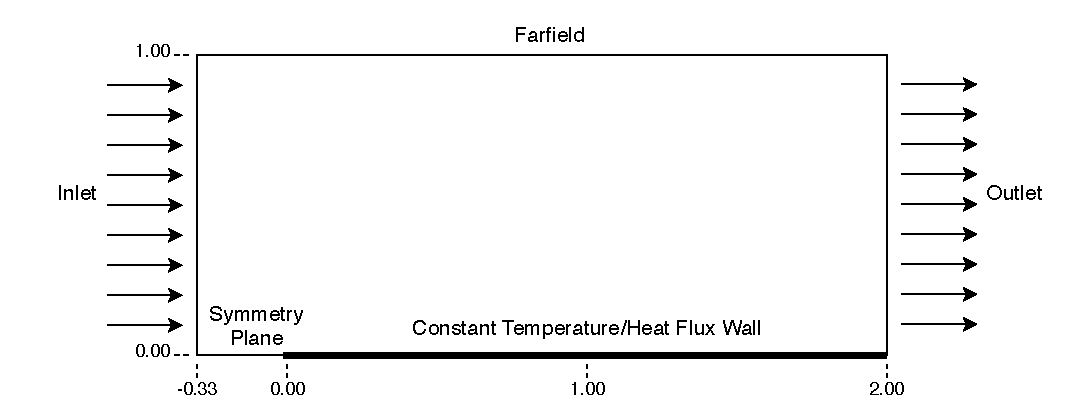
\includegraphics[width=0.8 \textwidth]{Error/FlatPlate.pdf}
  \caption{Schematic of the flat plate case.}
  \label{fig:Plate_Domain}
\end{figure}

The length of the flat plate is $L = 2.0$ m to achieve a Reynolds number comparable to the DNS results. This also removes any influence of the outlet boundary on the results in the interior domain of interest. The flat plate begins at $x = 0.0$ and has a lead-in distance of $0.33$ m to limit the influence of the inlet boundary condition. These dimensions correspond to a non-dimensional domain size of $Lx = 167~\delta$ and $Ly = 71.5~\delta$, with a lead-in of $L_i = 23.6~\delta$, based on the boundary layer thickness at $x = 1$ m from the leading edge ($\delta = 13.9$ mm). Table \ref{tbl:test-cases} summarizes the three conditions. They are: (1) a Mach 2.5 flow over an adiabatic wall $(T_w/T_r = 1)$, (2) a Mach 5.86 flow with low/moderate heat transfer at the wall $(T_w/T_r = 0.76)$, and (3) a Mach 5.84 flow with high heat transfer at the wall $(T_w/T_r = 0.25)$. The heat transfer cases are studied using both a constant wall temperature and heat flux boundary conditions.

%\begin{comment}
%The following test cases are ultimately investigated in this study,
%\begin{enumerate}
%\item \textbf{Supersonic/Hypersonic Flat Plate}
%  \begin{itemize}
%    \item Mach 2.5 and Mach 5.86
%    \item Adiabatic wall, and low/medium/high heat transfer at wall
%    \item SA and k-w SST turbulence models
%    \item Various $Y^+$ values
%    \item Standard Wall models and low-Re models
%  \end{itemize}
%  \item \textbf{Supersonic Wedge}
%  \begin{itemize}
%    \item Mach 2 and Mach 5
%    \item Adiabatic wall, and low/medium/high heat transfer at wall
%    \item SA and k-w SST turbulence models
%    \item Standard Wall models and low-Re models
%  \end{itemize}
%\end{enumerate}
%\end{comment}


\begin{table}
\centering
\caption{Summary of test cases.}
\label{tbl:test-cases}
\begin{tabular}{|l|ccccl|}
\hline
\multicolumn{1}{|c|}{\multirow{2}{*}{\textbf{Test Cases}}} &
  \multicolumn{5}{c|}{\textbf{Freestream conditions}} \\ \cline{2-6} 
\multicolumn{1}{|c|}{} &
  \multicolumn{1}{c|}{$U_\infty$ [m/s]} &
  \multicolumn{1}{c|}{$T_\infty$ [K]} &
  \multicolumn{1}{c|}{$\rho_\infty$ [kg/m$^3$]} &
  \multicolumn{1}{c|}{$T_{w}$ [K]} &
  \textbf{$T_{w}/T_{r}$} \\ \hline
\textbf{Mach 2.5 - No wall cooling} &
  \multicolumn{1}{c|}{823.6} &
  \multicolumn{1}{c|}{270.0} &
  \multicolumn{1}{c|}{0.10} &
  \multicolumn{1}{c|}{568.0} &
  1.0 \\ \hline
\textbf{Mach 5.86 - Low wall cooling} &
  \multicolumn{1}{c|}{870.4} &
  \multicolumn{1}{c|}{55.0} &
  \multicolumn{1}{c|}{0.043} &
  \multicolumn{1}{c|}{300} &
  0.76 \\ \hline
\textbf{Mach 5.84 - High wall cooling} &
  \multicolumn{1}{c|}{869.1} &
  \multicolumn{1}{c|}{55.2} &
  \multicolumn{1}{c|}{0.044} &
  \multicolumn{1}{c|}{97.5} &
  0.25 \\ \hline
\end{tabular}
\end{table}

\subsection{Test case 2: Supersonic Wedge}\label{sec:supersonicWedge}
A supersonic wedge is considered to study a slightly more complex case with a high-speed turbulent boundary layer with a pressure gradient. The wedge has an angle of $\theta_w = 15~\deg$. Previous numerical studies of supersonic flows over a wedge have been conducted \cite{Wu2007,Wagner2018}, but no DNS simulation nor detailed experimental data, such as boundary layer profiles, are available for the non-adiabatic wall supersonic wedge case \cite{ROY2006469}. Thus, the results of this test case cannot be assessed against a benchmark. Instead, the variation among the solvers is assessed for the supersonic wedge case. The case configuration is shown in Figure \ref{fig:Wedge_Domain}. Similar to the flat plate boundary layer case, a symmetry (slip) plane is added in front of the non-slip wall to avoid a separation zone at the corner. The analytical solution to the adiabatic supersonic wedge oblique shock angle can be found in the literature \cite{anderson2003, Gregory-Smith1983}. Similar to the flat plate case, three simulations are conducted: (1) a Mach 2.5 flow over an adiabatic wall, (2) a Mach 5 flow with low and  (3) high heat transfer at the wall. Both heat transfer cases are simulated with a constant temperature wall.

\begin{figure}
\centering
  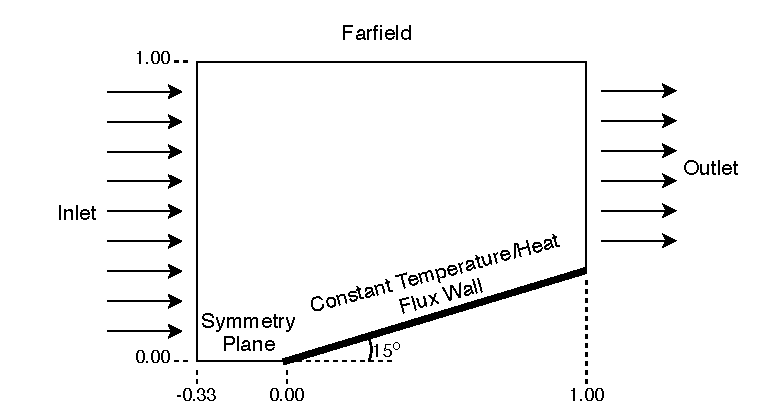
\includegraphics[width=0.6\textwidth]{Error/Wedge.pdf}
  \caption{Wedge case description.}
  \label{fig:Wedge_Domain}
\end{figure}



\section{Mesh and Simulation Setup}
The 2D (and quasi-3D) structured mesh of the flat plate and wedge configurations are created using Pointwise and OpenFOAM's \texttt{blockMesh} utility. A quasi-3D mesh is used in OpenFOAM and ANSYS CFX simulations due to the solvers' inability to use a truly two-dimensional mesh; in the present quasi-3-D cases, only one cell is used in the $z$-direction. The mesh is refined at the wall for a $Y^+ < 1$ to use the high-resolution turbulence model of the $k-\omega$ SST model.  The maximum $Y^+$ across all simulations and over all the computational domain is $Y^+ = 0.4$. The cell-to-cell expansion ratio at the bottom of the domain is $1.1201$. The mesh is also refined in the $x$-direction at $x=0$ m to properly capture the complex flow characteristics at the leading edge of the flat plate and the wedge. The cell-to-cell expansion ratio in the streamwise direction at $x=0.00$ is $1.02234$. Figure \ref{fig:Flat_Plate_Mesh}  shows the meshes used in the flat plate and wedge configuration, respectively. A grid independence study, discussed below, shows good independence of solution from grid sizing and convergence of solution results \ref{fig:Plate_Grid_Conv}. 

\begin{figure}
\centering
  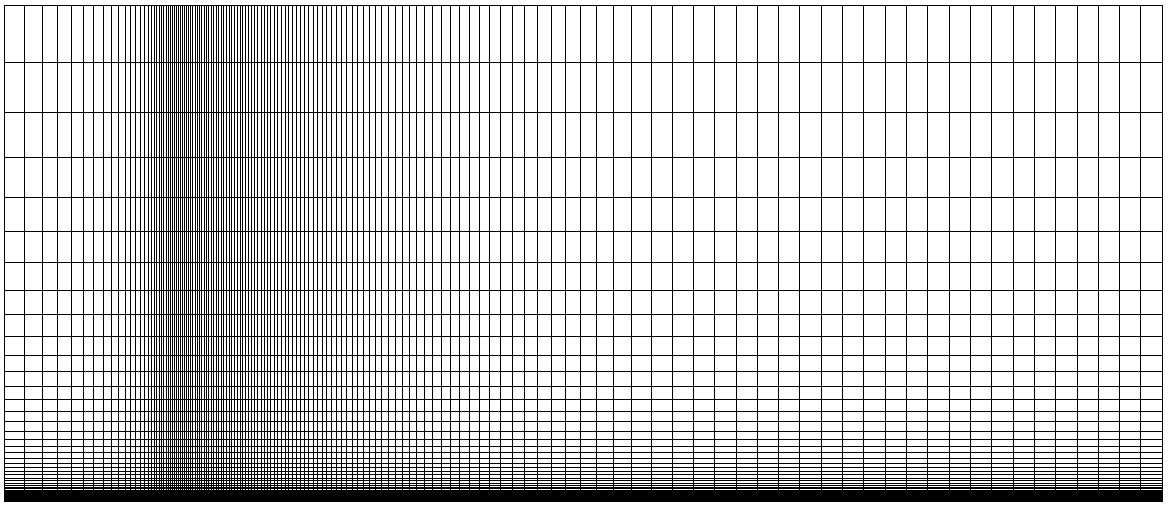
\includegraphics[width=0.4\textwidth]{Error/Plate_Medium.png}
  \hspace{1cm}
    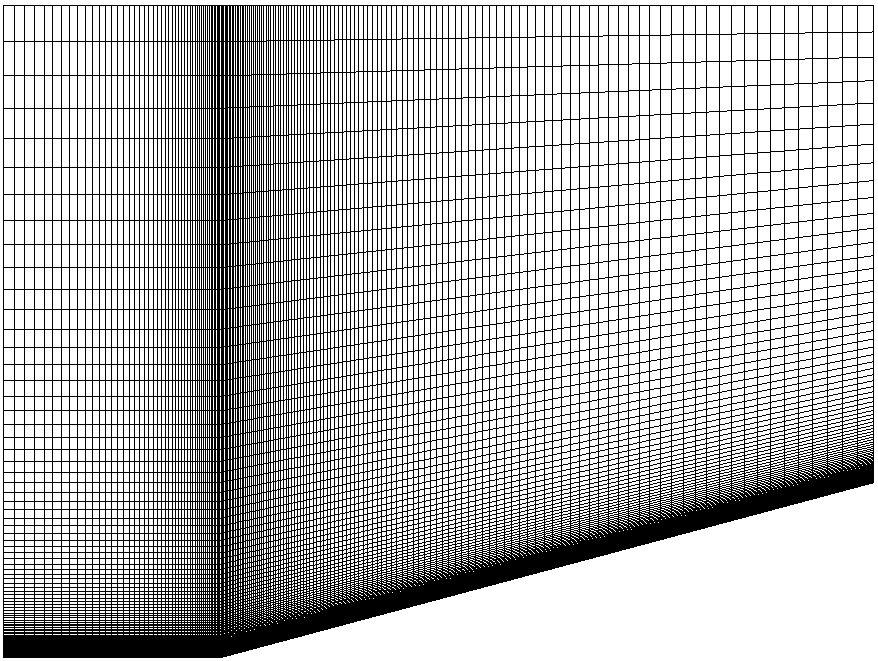
\includegraphics[width=0.3\textwidth]{Error/wedge_fine.png}
  \caption{Flat plate (left) and the wedge (right) mesh for the medium mesh.}
  \label{fig:Flat_Plate_Mesh}
\end{figure}
%\begin{figure}
%\centering
%  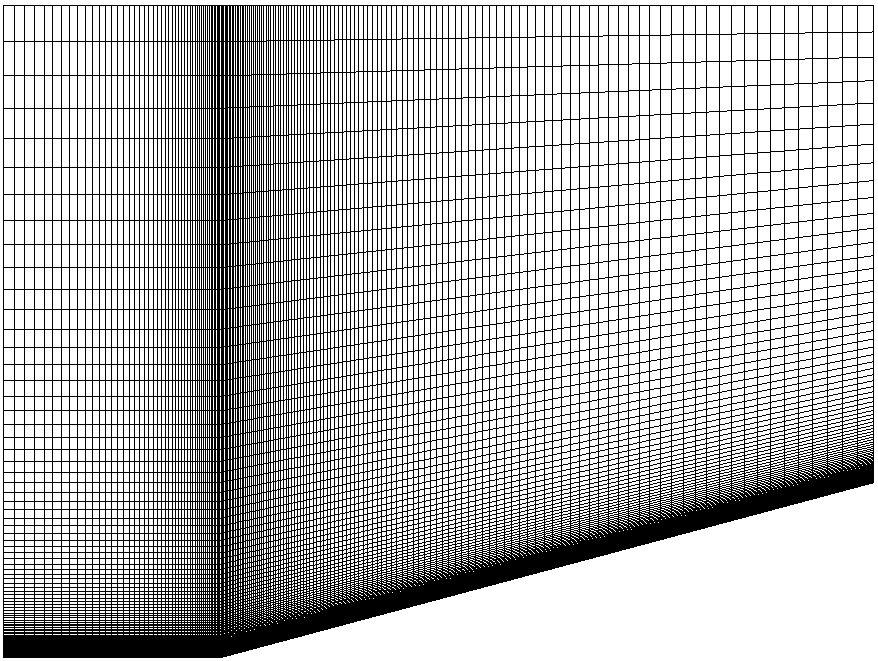
\includegraphics[width=0.3\textwidth]{Error/wedge_fine.png}
%  \caption{Wedge mesh configuration.}
%  \label{fig:Wedge_Mesh}
%\end{figure}


\subsection{Boundary Conditions}
Every solver has its own ``best-practice" for declaring domain boundary conditions for high-speed flows. Table \ref{tab:BC_comp} shows the boundary conditions used for all the four solvers. For clarity, the specific terminology used in each solver is adopted. For additional information on the implementation of these boundary conditions, the reader should consult the user guides for these codes \cite{SU2Code_userguide, Ansys_userguide, Openfoam_userguide, SiemensPLM}.

%Furthermore, in \texttt{rhoCentralFoam} the turbulent viscosity close to the wall is calculated by the \texttt{NuTSpalding Wall Function}, with $k$ diminishing to $0$, and $\omega$ approaching a very large value ($\sim 1E9$). NOT SURE IF I SHOULD INCLUDE THIS, SINCE IT SAYS THIS IN DOCUMENTATION

\begin{table}
\centering
\caption{Boundary Conditions Comparison}
\label{tab:BC_comp}
\begin{tabular}{|l|c|c|c|c|c|c|}
\hline
\multicolumn{1}{|c|}{\multirow{2}{*}{\textbf{Solver Suite}}} &
  \multicolumn{6}{c|}{\textbf{Domain Boundary Conditions}} \\ \cline{2-7} 
\multicolumn{1}{|c|}{} &
  \textbf{Inlet} &
  \textbf{Outlet} &
  \textbf{Symmetry} &
  \textbf{Farfield} &
  \textbf{Wall} &
  \textbf{\thead{Front/\\Back (3D)}} \\ \hline
SU2       & \thead{Supersonic\\ Inlet} & Outlet          & Symmetry & Outlet    & No-slip & - \\ \hline
OpenFOAM  &  \thead{Fixed\\ Value}     & \thead{Zero\\ Gradient}   & \thead{Symmetry\\ Plane} & \thead{Zero\\ Gradient} & No-slip &  Empty \\ \hline
ANSYS CFX &  \thead{Inlet\\ (Supersonic)}  & \thead{Outlet\\ (Supersonic)} &  Symmetry &   Symmetry   & No-slip &  Symmetry  \\ \hline
Star-CCM+ & Freestream       & \thead{Pressure\\ Outlet} & Symmetry & Freesteam & No-slip & - \\ \hline
\end{tabular}
\end{table}


\subsection{Solution Validation}
A validation is conducted to assess the convergence behavior and mesh independence for the present cases.

\subsubsection{Convergence}
Due to the inherent differences in the algorithmic and physical model, each solver has its own 'best-practice' to maintain stability and achieve steady-state convergence. The classical Courant–Friedrichs–Lewy (CFL) convergence condition needs to be satisfied to maintain numerical stability for explicit time integration schemes. The CFL condition is defined as,
\begin{align}
    Co={\frac  {c\,\Delta t}{\Delta x}}\leq Co_{\max }
\end{align}
where $c$ is the speed of sound, $\Delta t$ is the time step, $\Delta x$ is the smallest grid element length, and $Co$ is the Courant Number. Although explicit solvers need to stay under the CFL limit of $1$, implicit solvers can be accelerated by using a CFL limit much greater than unity because they are unconditionally stable. In Star-CCM+ and SU2, a Courant Number ramp is used to speed up convergence because they are all implicit solvers. The solvers are initially run at a CFL limit of $0.2 - 0.7$ is initially and ramps up to a CFL limit of $30$. As the simulations are run to steady-state, the CFL number does not impact the final solution.
%Figure \ref{fig:CFL_ramp} shows a typical Courant number ramp employed in the solvers. 

ANSYS CFX does not allow the definition of an explicit CFL number limit, and instead uses of a local time scale factor for convergence acceleration. CFX simulations are conducted using a local timescale factor of 5 until convergence, and then restart with a physical timescale of $0.0008s$, as recommended in the CFX user guide \cite{Ansys_userguide}. 

Since \texttt{rhoCentralFoam} is a transient solver that uses a central scheme, it is thus limited by the $Co \leq 0.5$ condition unique to central schemes \cite{Greenshields2010}. \texttt{rhoCentralFoam} simulations are run using a constant Courant number of $Co = 0.4$. 
%Since \texttt{rhoCentralFoam} is a transient solver, the converged simulation results are time-averaged, over a sufficiently large time domain, in a post-processing step. 


The convergence of the simulation is assessed in the following three ways:
\begin{enumerate}
    \item \textbf{Numerical Residuals} - The maximum normalized residuals for the steady-state solvers settled below $1 \times 10^{-7}$ for velocity, temperature, and turbulence quantities. In SU2, the flat plate RMS residuals are below $1 \times 10^{-11}$, and in Star-CCM+ and ANSYS CFX, the RMS residuals are below $1 \times 10^{-9}$. The RMS residual target for each time-step for OpenFOAM was set as $1 \times 10^{-13}$. The time-averaging process for OpenFOAM was conducted over 2000 iteration steps, although the time-averaging is not necessary as the flow eventually reaches a steady state with the transient solver. 
    \item \textbf{Solution Imbalances} - Mass, momentum and energy must be conserved through the simulation domain. The difference between the inlet mass flow and outlet mass flow must be balanced when reaching convergence (similarly for momentum). This is quantified by writing solution imbalances during run-time in the execution windows for all the solvers tested.
    \item \textbf{Stability of Quantities} - No oscillations are observed with the coefficient of drag, wall heat transfer rate, and coefficient of pressure values while reaching convergence. This was a qualitative assessment, conducted for SU2 by plotting the surface-average quantity history in the post-processing step. 
    %shown in Figure \ref{}. 
    Similarly, real-time plotting of the performance parameters were done on ANSYS CFX and Star-CCM+. The stability of performance parameters for OpenFOAM was qualitatively assessed by probing the point of interest in \texttt{paraFOAM} and noting the maximum variation between time steps. 
\end{enumerate}

%\begin{figure}
%\centering
%  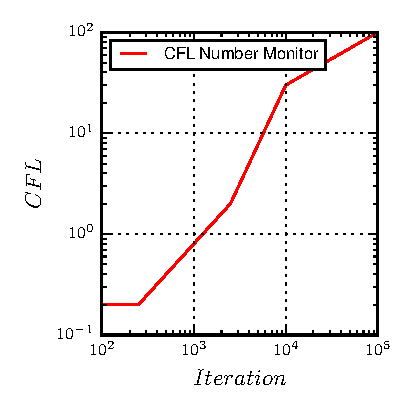
\includegraphics[width=0.4\textwidth]{Error/CFL_RAMP.pdf}
%  \caption{A typical CFL ramp used in the present study.}
%  \label{fig:CFL_ramp}
%\end{figure}

\subsubsection{Grid Independence}
A grid-independence study is conducted to understand the influence of grid resolution on the result. The coarsity of grids is by calculated using the following relationship,
\begin{align}
    N = 2^{n} m + 1
\end{align}
where $N$ is the number of mesh elements in a given coordinate direction, $n$ is the number of ``levels" of mesh refinement, and $m$ is a pre-determined integer that can differ in each coordinate \cite{NASASpatialValidation}. In this case, $n = 0, 1, 2, 3$ and $m_x = 34$ and $m_y = 24$. Table \ref{tbl:Plate_Grid_Metrics} shows the statistics of the meshes used in the grid-independence study. The grid independence checks are conducted on SU2 using a Mach 5 flow, with a constant temperature wall boundary condition set at the recovery temperature of the fluid $(T_w/T_r = 1)$.

\begin{table}
\caption{Flat Plate Mesh Statistics}
\label{tbl:Plate_Grid_Metrics}
\centering
\begin{tabular}{|l|c|c|c|c|}
\cline{1-5}
\textbf{Mesh} &
  \textbf{\begin{tabular}[c]{@{}l@{}}$N_y$\end{tabular}} &
  \textbf{\begin{tabular}[c]{@{}l@{}}$N_x$\end{tabular}} &
  \textbf{\begin{tabular}[c]{@{}l@{}}Total Elements\end{tabular}} &
  \textbf{Max. $Y^+$} 
   \\ \hline \hline 
Very Coarse & 25 & 35 & 875 & 7   \\ \cline{1-5}
Coarse & 49 & 69 & 3381 & 3   \\ \cline{1-5}
Medium & 97 & 137 & 13,289 & 0.4   \\ \cline{1-5}
Fine   & 193 & 273 & 52,689 & 0.2  \\ \cline{1-5}
\end{tabular}
\end{table}

Figure \ref{fig:Plate_Grid_Conv} shows the computed normalized wall-normal velocity and temperature profiles for increasing mesh resolution. Also included is the Stanton number at the constant-temperature wall. The results converge towards the fine mesh. The medium mesh with $135 \times 97$ elements is used in the present study, and is considered grid-independent.

\begin{figure}
\centering
  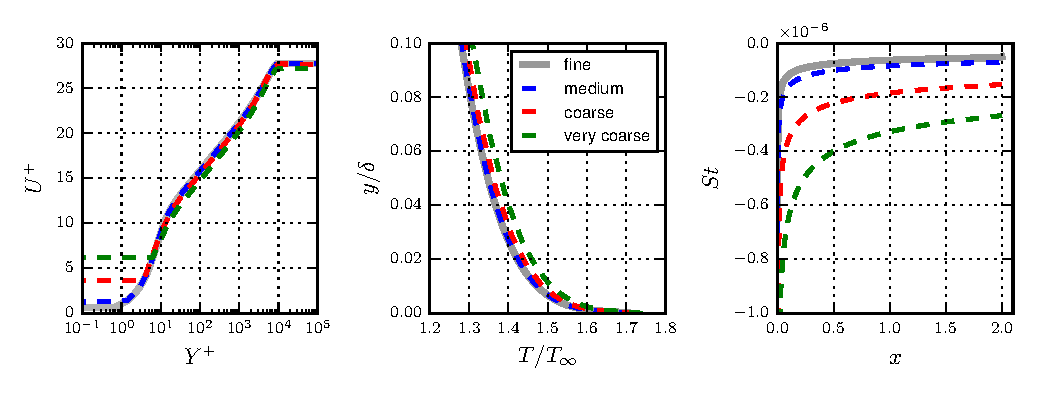
\includegraphics[clip, trim=0cm 0.5cm 0cm 0.2cm, width=\textwidth]{Error/Plate_Grid_conv.pdf}
  \caption{Flat plate grid convergence study.}
  \label{fig:Plate_Grid_Conv}
\end{figure}

\section{Results and Discussion}\label{sec:res}
This section presents the comparison of the four codes used in this study. The RANS codes are first compared to the mean quantities of equivalent DNS studies. Finally, the codes are compared with each other to quantify the variation between them, for both constant temperature wall and constant wall heat flux conditions. 

\subsection{Solver Accuracy}
The commercial and open-source RANS solvers in the study are first assessed on their general ability to accurately capture the boundary layer and wall parameters in high-speed cold-wall flows. A similar study was conducted by Huang et al. \cite{Huang2019} in 2019 with greater emphasis on the turbulence model's ability to accurately capture the turbulence statistics near the wall. Conversely, this study emphasizes the error assessment among the solvers to simulate cold-wall, high-speed turbulent boundary layer flows.  %As mentioned previously, all the simulations in this study use Menter's $k-\omega$ SST  for turbulence modelling. 
The wall-normal profiles are extracted at $x = 0.45$ to achieve a similar momentum thickness Reynolds number ($Re_{\theta}$) as the DNS simulation, and in this case, $Re_{\theta} = 4845$. $Re_{\theta}$ was calculated in the post-processing step using Equation \eqref{eqn:Re_theta}.


Figure \ref{fig:Plate_RANS2} shows the normalized wall-normal velocity, temperature, and density contours for a Mach 2.5 zero-pressure gradient flat plate case, with no wall cooling. The velocity magnitude, temperature, and density are normalized using freestream values. %In this test case, the freestream temperature is $T_{\infty} = 270.0K$ and the wall temperature is set at a constant $T_w = 568.0K$. 
Overall, all the tested solvers display reasonable agreement with the DNS results. Even in a low-supersonic, no-wall cooling scenario, the wall-normal temperature profile is over-estimated in all codes in the near-wall region ($y/\delta \sim 0.1$). This may be due to an over-prediction of the eddy viscosity very close to the wall, which results in more thermal diffusion through the boundary layer. Figure \ref{fig:Plate_RANS2_Cd} shows the coefficient of pressure, coefficient of drag, and the Stanton number for the Mach 2 case with no wall cooling. Although a constant wall temperature boundary condition was enforced based on the wall-to-recovery temperature of the fluid $T_w/T_{aw} = 1$, the temperature of the fluid behind the shock wave differs slightly from the freestream temperature of fluid $T_{\infty}$, resulting in a non-zero heat flux computed at the wall. 

Similar agreement is shown in Figure \ref{fig:Plate_RANS6AD} for a Mach 5.86 case with low wall cooling. 
%The wall temperature is set at a constant $T_{w} = 300.0K$ while the freestream temperature is $T_{\infty} = 55.0K$, resulting in a wall temperature to recovery temperature of  $T_w/T_{aw} = 0.75$. 
Note that the effect of an increased Mach number and a slightly non-adiabatic wall has a minor impact on the accuracy of the results. Figure \ref{fig:Plate_RANS6} shows the wall-normal profiles for a Mach 5.84 case with a high wall cooling case. 
%The freestream temperature for this case is $T_{\infty} = 55.0K$, while the wall temperature is $T_w = 97.5K$, which produces a wall temperature to recovery temperature ratio of  $T_w/T_{aw} = 0.25$. 

All of the codes deal with the large thermal gradient similarly, and none of them are able to accurately capture the boundary layer. Particularly, the thermal boundary layer is grossly over-estimated throughout the boundary layer; see Figure \ref{fig:ThermalBL}. The maximum temperature in the viscous sub-layer, at $y = 0.0002$ ($y/\delta = 0.1$), is also over-predicted by a significant margin. The thermal diffusion in the boundary layer is far greater in the RANS codes as compared to the DNS simulation. The maximum normalized wall distance for the mesh in this simulation is $Y^+ = 0.4$,  and further simulations with lower $Y^+$ values have shown to improve this disparity; however, the impact is only marginal. 


\begin{figure}
\centering
    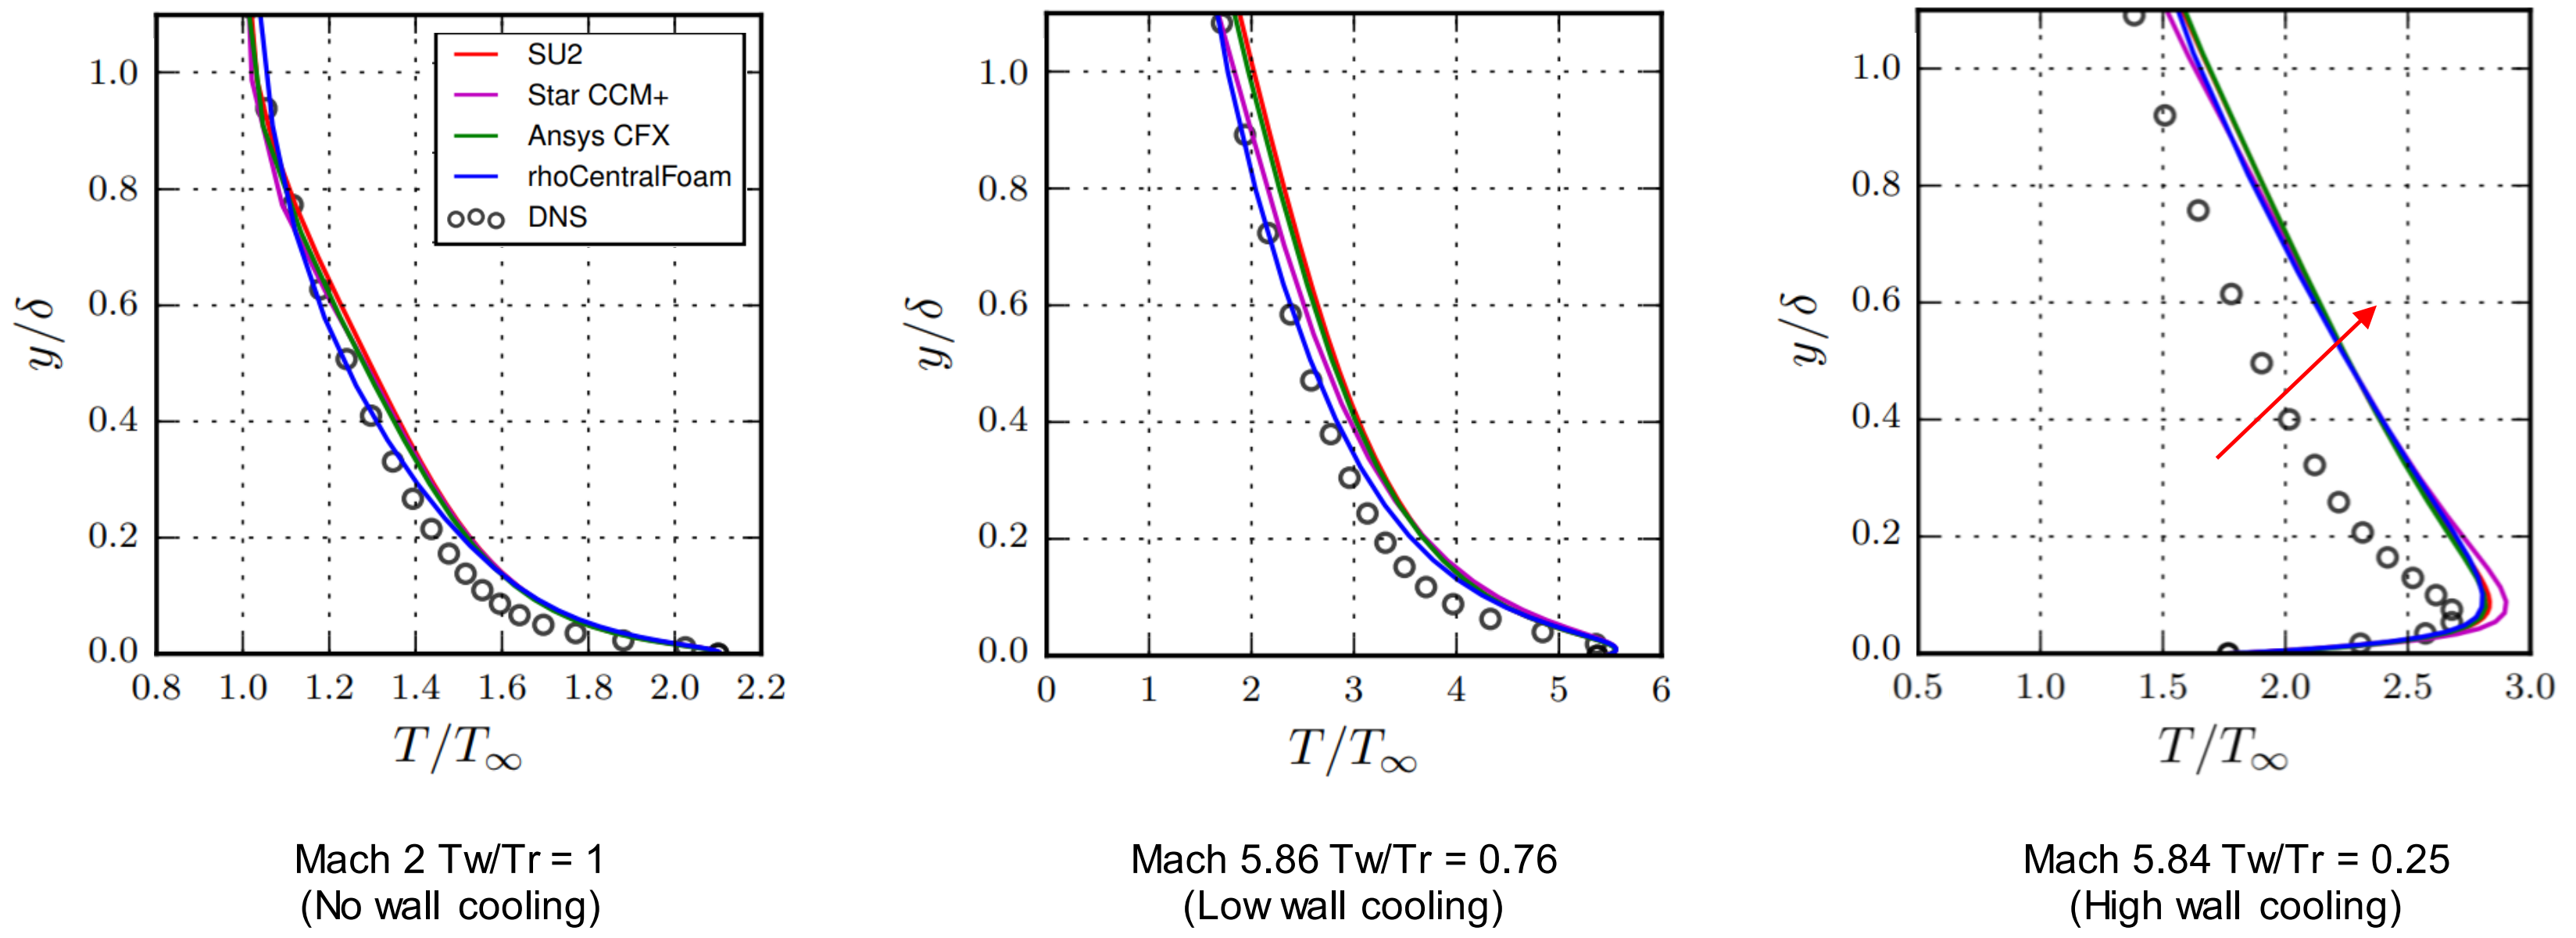
\includegraphics[width=\textwidth]{CHT/Thermal_Boundary_Layer.png}
  \caption{Normalized thermal boundary layer for with constant wall temperature boundary condition, compared to DNS simulations of Zhang et al. \cite{Zhang2018DNS}. The thermal boundary layer is captured less accurately with increasing Mach number, as shown by the red arrow.}
  \label{fig:ThermalBL}
\end{figure}

Figures \ref{fig:Plate_RANS6AD_Cd} and \ref{fig:Plate_RANS6_Cd} show the wall quantities for the Mach ~6 cases with low and high wall cooling, respectively. The DNS results for the Stanton numbers are also plotted therein. The Stanton numbers computed for all the solvers tested show similar prediction to the DNS, even in highly non-adiabatic wall cases. This supports similar results obtained by Huang et al \cite{Huang2019}. The effect of Sarkar's compressibility correction (a default correction applied by Star-CCM+) is shown in these figures as dotted lines, which shows superior prediction in the wall heat flux in the low-wall cooling case. However, the compressibility correction performs poorly for the highly-cooled wall scenario. This could result from an under-prediction of turbulence dissipation introduced by the limiter function based on the turbulent Mach number; see Equation \eqref{eq:comp_corr_1} and \eqref{eq:comp_corr_2}.

\subsection{Solver Comparison}
The codes are subsequently compared against each other to quantify the average variation among them. They are also compared in terms of key performance parameters, such as the coefficients of pressure, coefficient of drag, and the heat transfer at the wall. The codes are first compared on a fixed wall temperature case, and then on a case with a fixed wall-heat flux.

\subsubsection{Constant Temperature Wall}
\label{sec:const_temp_wall}
 The difference between the solvers in the boundary layer performance parameters is computed. The wall-normal velocity, density, and temperature profiles are integrated from the bottom wall to $95\%$ of the boundary layer thickness for all solvers. The integrated wall-normal values is averaged among the four solvers. The average and maximum percentage difference between the solvers is computed. The solver variation metrics are computed as follows,

\begin{align}
        &Avg. \: Relative =   \frac{\sum_{n=1}^4 \left( \left| \frac{\sum_{n=1}^4 \bar{F}_n}{4} - \bar{F}_n \right| \right)}{\sum_{n=1}^4 \bar{F}_i} \times 100\%         \label{eq:var_avg_rel} \\
        %Maximum \: Relative &=   \frac{max\left( \left| F_1 - F_2 \right|, \left| F_1 - F_3 \right|, \left| F_1 - F_4 \right|, \left| F_2 - F_3 \right|, \left| F_2 - F_4 \right|, \left| F_3 - F_4 \right| \right)}{\sum_{n=1}^4 F_n} \times 100\% \\
        &Max. \: Absolute =   \max\left( \left| \bar{F}_i - \bar{F}_j \right| \right)   && i \neq j \label{eq:var_max_abs} \\
        &Max. \: Relative =   \frac{\max\left( \left| \bar{F}_i - \bar{F}_j \right| \right)}{\sum_{n=1}^4 \bar{F}_n} \times 100\%   && i \neq j \label{eq:var_max_rel}         
\end{align} 
where $n$ represents the solver index (ranging from $1$ to $4$, since the study compares four solvers), and $F$ is an arbitrary wall-normal property that is numerically integrated through the boundary layer, 
\begin{align}
        \bar{F}_n &= \int_{y=0}^{y=\delta} F_n(y) dy
\end{align}

A similar approach is taken for the coefficient of pressure, skin-friction coefficient, and the Stanton number. However, it is integrated along the surface of the wall instead. The effects from the leading edge of the flat plate and the domain outlet are omitted in the solver variation calculations. The omitted regions are displayed as dark grey boxes in Figures \ref{fig:Plate_RANS2_Cd},  \ref{fig:Plate_RANS6AD_Cd}, and \ref{fig:Plate_RANS6_Cd}. These values are tabulated in Table \ref{tab:ConstT_comp} for the constant temperature wall flat plate cases. Note that the numerical values of the maximum absolute variation using this method are only used as a numerical tool to compare absolute values across solvers. Furthermore, the variation calculated using this method is subject to the bounds of integration, i.e. the calculated variation becomes smaller as the integrated length increases. 

%The quantification of localized maximum variations will be quantified in a later study.

Figures \ref{fig:Plate_RANS2}, \ref{fig:Plate_RANS6AD}, and \ref{fig:Plate_RANS6} shows that the solver variation in the wall-normal velocity, pressure, and density profiles for a constant temperature wall are relatively small, regardless of wall-cooling rates or Mach number. All the solvers tested produce similar results, confirming that the essential physics in the near-wall region of cold-wall supersonic boundary layer flows are adequately captured in all codes. It is noted that pressure-based solvers (ANSYS CFX) and density-based solvers do not display any significant difference even at these extreme regimes. Particularly, \texttt{rhoCentralFoam}, deviates the most from the other solvers in the study. 
%which can be attributed to the transient nature of the solution, as compared to the steady-state solutions provided by all the other codes. 
Furthermore, unlike the other codes, \texttt{rhoCentralFoam} has little information on solver setup in high-speed flows, and a more optimal simulation setup may produce less deviation. 


%On the other hand, not all variation in the boundary layer is equal. For example, 
Variation near the wall in the viscous sublayer is largely more important than variation in the outer region of the boundary layer because most wall values and performance parameters are computed based on the first few grid elements close to the wall. Star-CCM+ displays one such deviation through an over-prediction of temperature in the viscous sublayer for the Mach $\sim$6 high wall cooling case (Figure \ref{fig:Plate_RANS6}), which is important to the calculation of the wall heat flux.
Key performance parameters such as the coefficient of pressure ($C_P$), coefficient of skin-friction drag ($C_f$), and the Stanton Number ($St$) are plotted along the flat plate wall in Figures \ref{fig:Plate_RANS2_Cd},  \ref{fig:Plate_RANS6AD_Cd}, and \ref{fig:Plate_RANS6_Cd} for the Mach 2.5 case, and $\sim$Mach 6 cases with low wall cooling and high wall cooling cases, respectively. As expected, the performance parameters calculated near the leading edge of the flat plate shows significant variation between the codes, and the variation becomes increasingly apparent with increased Mach numbers. %This is of course expected, since the leading edge of an infinitely thin plate is inherently under-resolved, and each solver deals with this feature differently. 
Similar to the wall-normal properties, the pressure and skin-friction coefficient values predicted across the four solvers show relatively little variation for the majority of the plate. The Stanton number, and by extension, the solver-computed heat flux at the wall, qualitatively shows the most variation, shown more clearly in Figure \ref{fig:Wallheatfluxplate}. The deviation between the Sarkar's compressibility corrected values and the other solver results increases significantly with increased Mach number and wall heat flux. 

\begin{figure}
\centering
    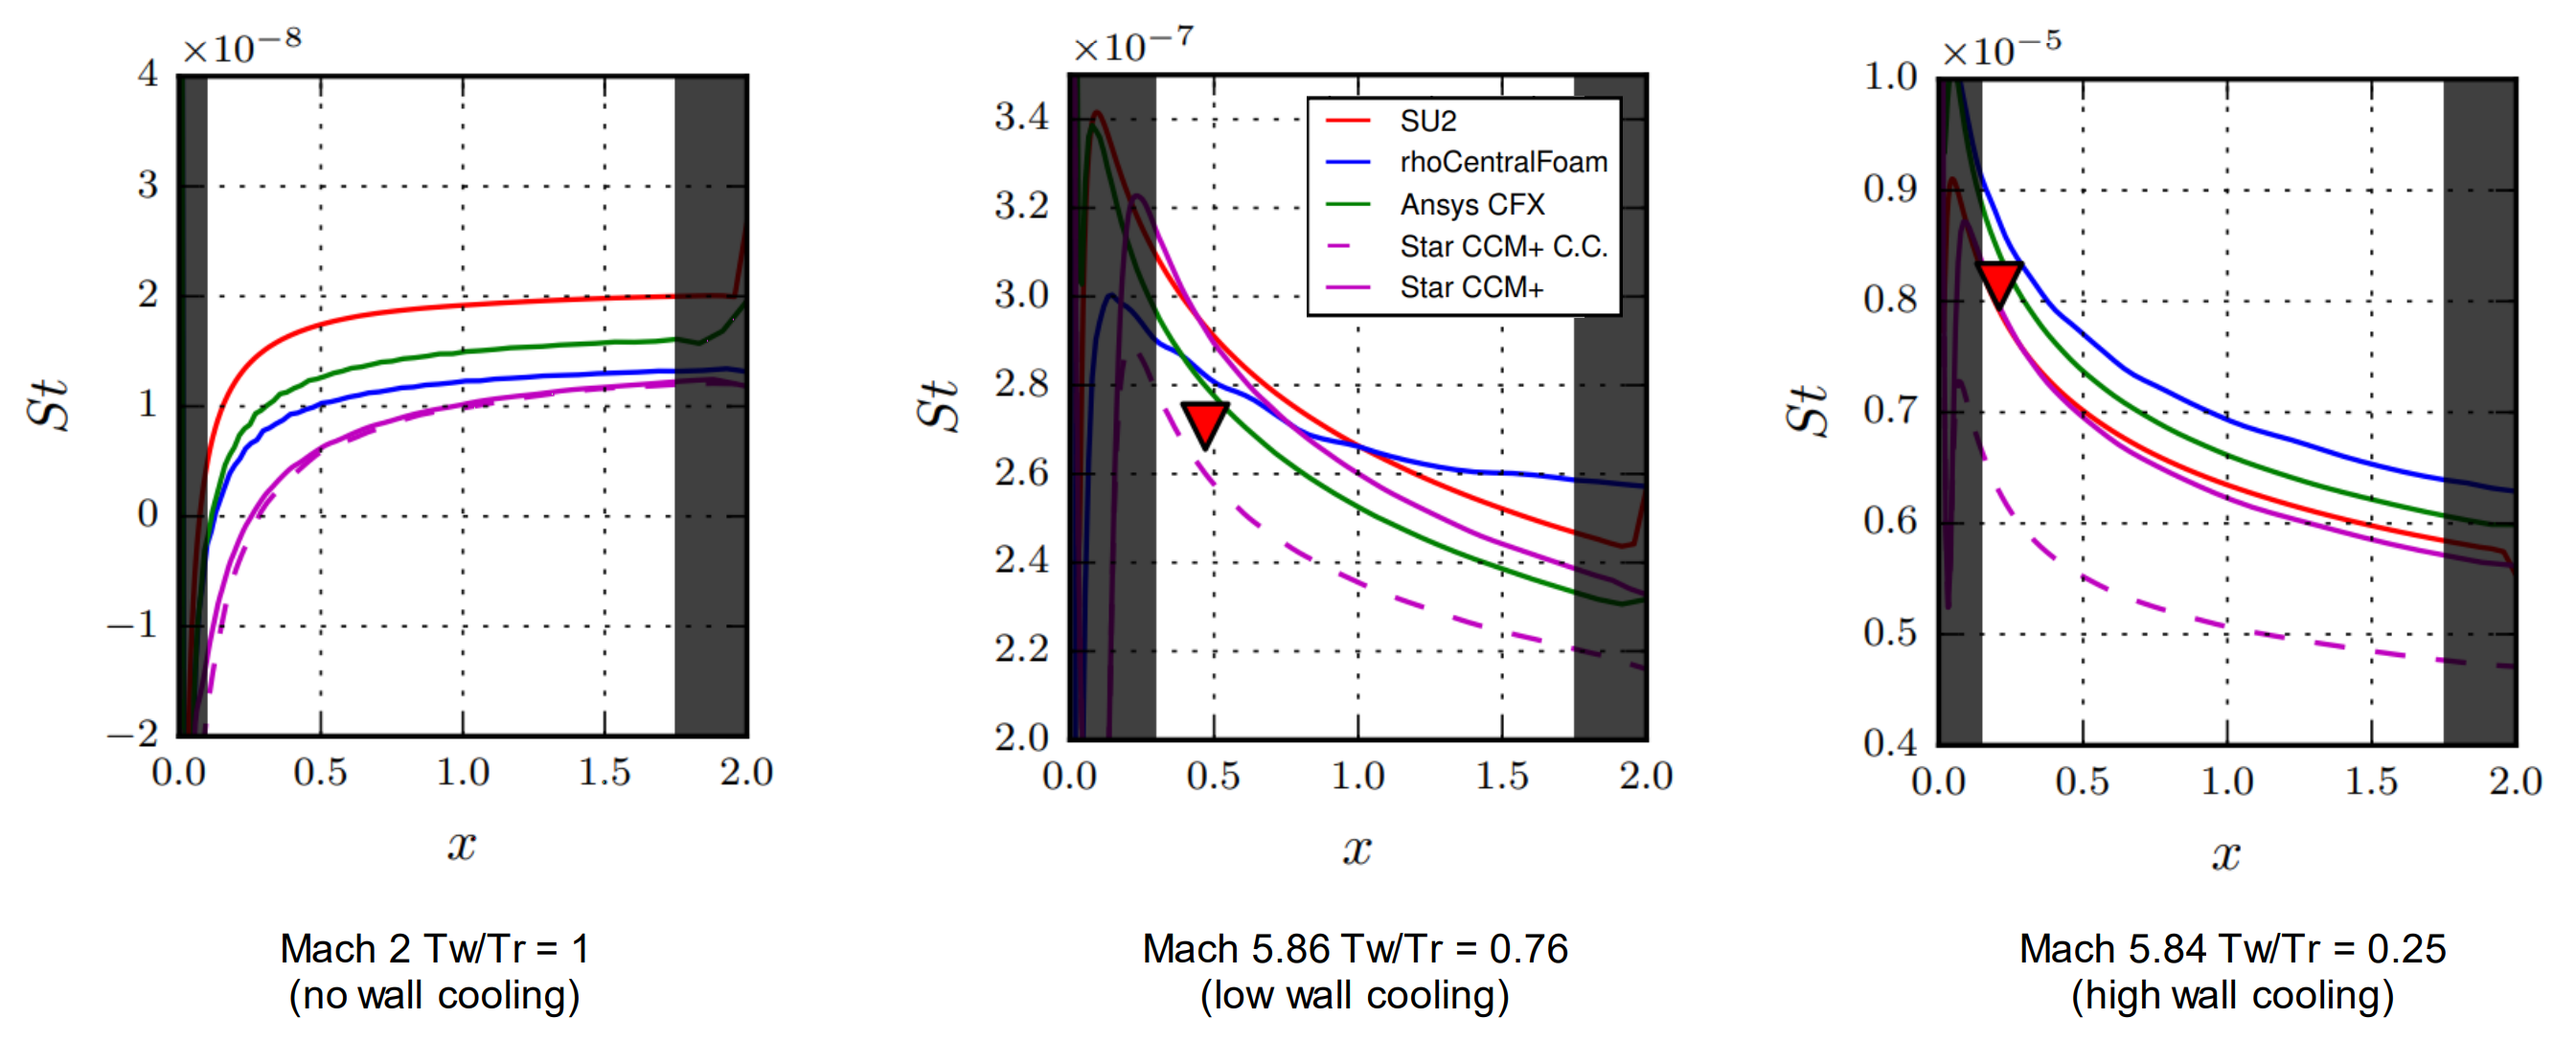
\includegraphics[width=\textwidth]{CHT/Wall_Heat_Flux.png}
  \caption{Solver comparison of normalized wall heat flux along the surface of the plate. The dotted line is Sarkar's compressibility correction. The red triangle represents DNS simulation results from Zhang et al. \cite{Zhang2018DNS}.}
  \label{fig:Wallheatfluxplate}
\end{figure}

The variation in the integrated wall-normal profiles and performance parameters for the constant temperature are quantified using Equations \eqref{eq:var_avg_rel}, \eqref{eq:var_max_abs}, and  \eqref{eq:var_max_rel} and are tabulated in Table \ref{tab:ConstT_comp}. Average variation between the solvers is around $2\% - 4\%$. The maximum relative variation between the integrated profiles however is much larger - as much as $\sim13\%$ for the normalized density profiles. However, the large average and maximum relative variations in the Stanton number for the Mach 2.5 case are artifacts of calculating relative changes close to zero because the heat flux for this test case tends towards zero. A more direct comparison can be attained by comparing the absolute values of these integrated variations, listed in Table \ref{tab:ConstT_comp} as ``Max. Abs." variations. Although these numbers do not have a physical interpretation, it can be used as an important tool for comparing the variation in the wall-normal profiles for each test case, where the temperature variation in the boundary layer holds the largest absolute variation for all the test cases. This can be partly explained by the integration bounds of the quantification approach ($95\%$ of boundary layer thickness) because the Prandtl number for the simulations are $0.71$ --- meaning the thermal boundary layer is larger than the velocity boundary layer. 

The absolute variation also shows a general trend - an increase in Mach number decreases the solver variation, displayed by a drop in average and maximum variation between the Mach 2.5 and Mach 5.86 simulation, and increasing wall cooling rates increases the maximum absolute variation between the solvers. However, three data points are not enough to confirm this trend, and a deeper investigation is needed to correlate Mach number and non-adiabatic wall effects on solver variation.

\begin{table}
\centering
\caption{Solver variation for a boundary layer on a flat plate with a constant temperature wall.}
\label{tab:ConstT_comp}
\begin{tabular}{|c|c|c|c|c|c|c|c|c|c|}
\hline
\multirow{2}{*}{\textbf{Prop.}} &
  \multicolumn{3}{c|}{\textbf{\begin{tabular}[c]{@{}c@{}}Mach 2.5\\ $T_w/T_{aw} = 1$\end{tabular}}} &
  \multicolumn{3}{c|}{\textbf{\begin{tabular}[c]{@{}c@{}}Mach 5.86\\ $T_w/T_{aw} = 0.75$\end{tabular}}} &
  \multicolumn{3}{c|}{\textbf{\begin{tabular}[c]{@{}c@{}}Mach 5.84 \\ $T_w/T_{aw} = 0.25$\end{tabular}}} \\ \cline{2-10} 
 &
  \textbf{\begin{tabular}[c]{@{}c@{}}Max.\\ Abs.\end{tabular}} &
  \textbf{\begin{tabular}[c]{@{}c@{}}Max.\\ Rel.\end{tabular}} &
  \textbf{\begin{tabular}[c]{@{}c@{}}Avg.\\ Rel.\end{tabular}} &
  \textbf{\begin{tabular}[c]{@{}c@{}}Max.\\ Abs.\end{tabular}} &
  \textbf{\begin{tabular}[c]{@{}c@{}}Max.\\ Rel.\end{tabular}} &
  \textbf{\begin{tabular}[c]{@{}c@{}}Avg.\\ Rel.\end{tabular}} &
  \textbf{\begin{tabular}[c]{@{}c@{}}Max.\\ Abs.\end{tabular}} &
  \textbf{\begin{tabular}[c]{@{}c@{}}Max.\\ Rel.\end{tabular}} &
  \textbf{\begin{tabular}[c]{@{}c@{}}Avg.\\ Rel.\end{tabular}} \\ \hline
\textbf{$U/U_{\infty}$}    & 4.20e-3 & $12.64\%$ & $3.89\%$  & 1.82e-3 & $13.09\%$ & $4.27\%$ & 3.27e-3 & $12.31\%$ & $3.36\%$ \\ \hline
\textbf{$\rho/\rho_{\infty}$} & 4.34e-3 & $13.09\%$ & $4.09\%$  & 1.34e-3 & $14.16\%$ & $6.76\%$ & 3.36e-3 & $12.51\%$ & $3.45\%$ \\ \hline
\textbf{$T/T_{\infty}$}    & 4.75e-3 & $12.75\%$ & $4.00\%$  & 5.10e-3 & $10.89\%$ & $4.26\%$ & 3.45e-3 & $11.08\%$ & $2.90\%$ \\ \hline
\textbf{$c_P$}  & 1.28e-2 & $3.4\%$  & $1.15\%$  & 2.17e-3 & $4.06\%$  & $1.50\%$ & 2.7e-3  & $5.18\%$  & $1.68\%$ \\ \hline
\textbf{$c_f$}  & 7.87e-5 & $2.46\%$  & $0.9\%$  & 7.98e-5 & $6.31\%$  & $1.73\%$ & 1.36e-4 & $8.21\%$  & $2.52\%$ \\ \hline
\textbf{$St$}   & 1.67e-8 & $69.6\%$  & $27.00\%$ & 2.76e-8 & $8.73\%$  & $2.37\%$ & 9.15e-7 & $11.68\%$ & $3.09\%$ \\ \hline
\end{tabular}
\end{table}


%Although the aximum relative (and average relative) variation between the solvers drops with the increased wall cooling in the Mach ~5.8 cases, the absolute variation between them generally increases. 
% The cause for this increase could be attributed to the differences in the implementation of near wall models and boundary conditions (usually derived from adibatic wall conditions) across the codes that become apparent when the wall becomes increasingly non-adiabatic. 

\subsubsection{Constant Wall Heat Flux}
A complementary study to Section \ref{sec:const_temp_wall} is conducted with a constant heat flux boundary condition enforced at the wall to observe any notable changes in the variation of the solvers. The physics, model, and numerical definitions are reused from each of the $\sim$Mach 6 constant temperature wall cases, with the exception of a constant heat flux boundary condition at the wall. Cases for heat flux values of $q_w = -2500 \frac{W}{m^2}$ and $q_w = -10,000 \frac{W}{m^2}$ are run across all the solvers for the flat plate cases, corresponding to a Stanton number of approximately $St = 3 \times 10^{-7}$ and $St = 7 \times 10^{-6}$ respectively. All the solvers are compared at $x=0.5$ for both the low and high wall cooling cases. Solution divergence was prevalent in \texttt{rhoCentralFoam} when a constant heat flux wall boundary condition was enforced.
This is because \texttt{rhoCentalFoam} does not have the ability to clip variables when experiencing negative temperatures and densities (common during the first few iteration steps). For this reason, the \texttt{rhoCentralFoam} simulation is run using a constant temperature wall condition until convergence, and the simulation is restarted with a constant heat flux boundary condition. However, \texttt{rhoCentralFoam} did not converge to a valid result for the $q_w = -10,000 W/m^2$ case, and is thus omitted in the plots and solver variation comparison.

\begin{figure}[htb]
\centering
    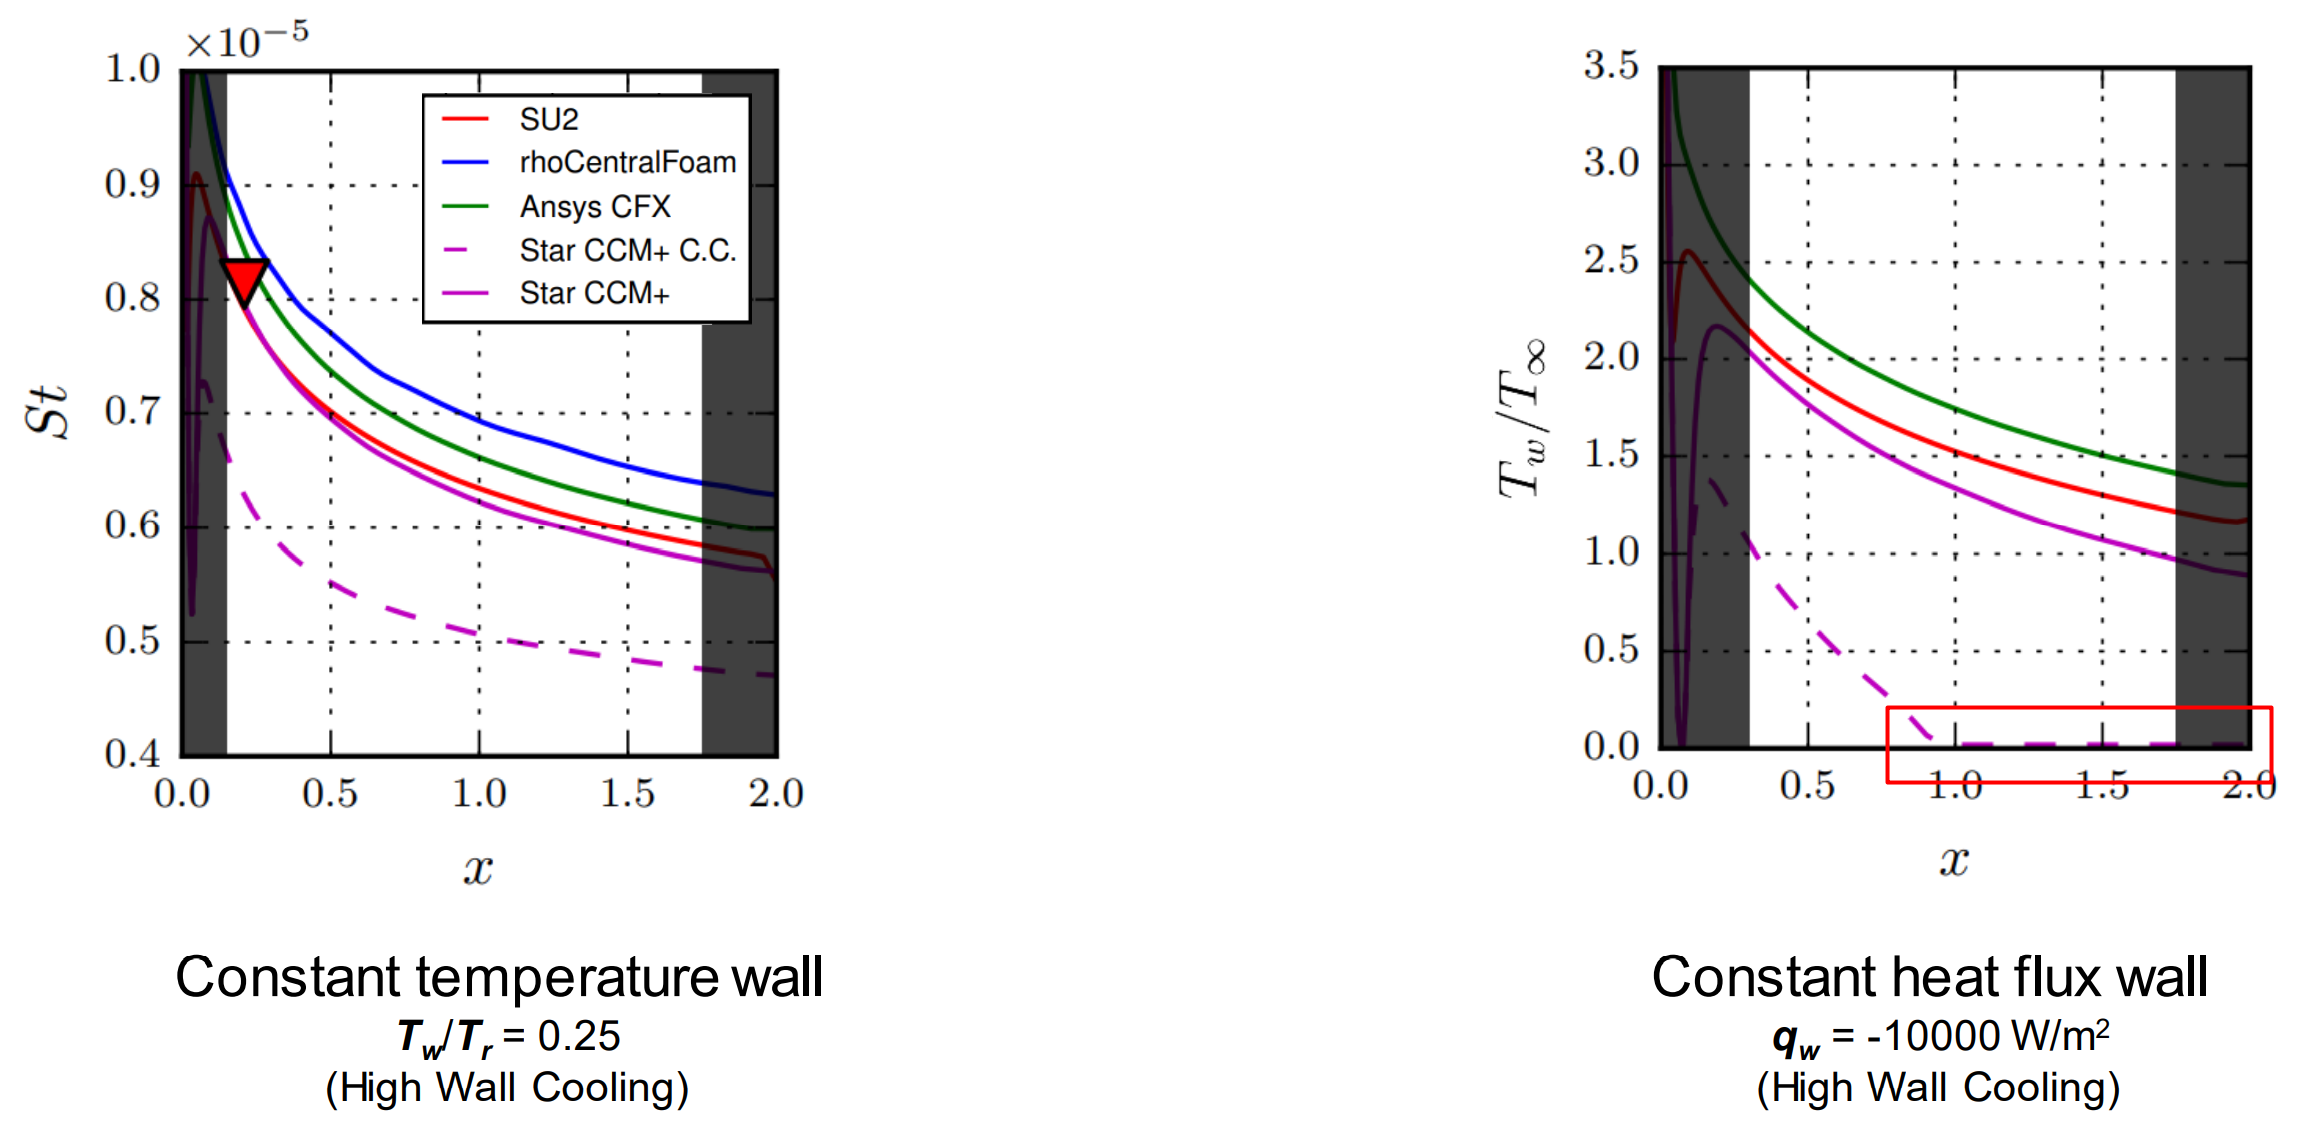
\includegraphics[width=0.9\textwidth]{CHT/Wall_Heat_Flux_2.png}
  \caption{Influence of wall boundary condition treatment on solver variation at Mach 6. The dotted line shows Sarkar's compressibility correction failing siginificantly for highly non-adiabatic walls, also producing non-physical values (red box).}
  \label{fig:Sarkar}
\end{figure}

Figures \ref{fig:Plate_RANS6HFLow} and \ref{fig:Plate_RANS6HFHigh} show the normalized wall-normal velocity, temperature, and density profiles for a complementary constant heat flux condition. The thermal and density profile in the viscous sublayer in both these cases vary significantly ($y/\delta \approx 0.01$). This variation is important in real-world engineering cases because minor differences in near-wall flow properties will have a significant impact on the predicted performance parameters. Figures \ref{fig:Plate_RANS6HFLow_Cd} and \ref{fig:Plate_RANS6HFHigh_Cd} confirm this, where it is visually apparent that the solver variation using a heat flux boundary condition is greater than the equivalent constant temperature wall cases, particularly with the wall temperature (shown more clearly in Figure \ref{fig:Sarkar}). Similar to the constant temperature wall cases, Sarkar's compressibility correction in Star-CCM+ fails in the $q_w = -10,000 W/m^2$ case and produces non-physical temperatures (see Figure \ref{fig:Sarkar}). This follows the trend that Sarkar's compressibility correction fails progressively for increasingly cooled walls. 


\begin{table}
\caption{Solver variation for a boundary layer on a flat plate with a constant heat flux at the wall.}
\label{tab:ConstHF_comp}
\centering
\begin{tabular}{|c|c|c|c|c|c|c|}
\hline
\multirow{2}{*}{\textbf{Prop.}} &
  \multicolumn{3}{c|}{\textbf{\begin{tabular}[c]{@{}c@{}}Mach 5.86\\ $St = 3E-7$\end{tabular}}} &
  \multicolumn{3}{c|}{\textbf{\begin{tabular}[c]{@{}c@{}}Mach 5.84\\ $St = 7E-6$\end{tabular}}} \\ \cline{2-7} 
 &
  \textbf{\begin{tabular}[c]{@{}c@{}}Max.\\ Abs.\end{tabular}} &
  \textbf{\begin{tabular}[c]{@{}c@{}}Max.\\ Rel.\end{tabular}} &
 \textbf{\begin{tabular}[c]{@{}c@{}}Avg.\\ Relative\end{tabular}} &
  \textbf{\begin{tabular}[c]{@{}c@{}}Max.\\ Abs.\end{tabular}} &
  \textbf{\begin{tabular}[c]{@{}c@{}}Max.\\ Rel.\end{tabular}} &
 \textbf{\begin{tabular}[c]{@{}c@{}}Avg.\\ Rel.\end{tabular}}\\ \hline
\textbf{$U/U_{\infty}$}    & 2.50e-3    & $13.2\%$  & $3.60\%$ & 3.32e-3    & $16.65\%$ & $4.98\%$ \\ \hline
\textbf{$\rho/\rho_{\infty}$} & 2.46e-3  & $15.70\%$ & $4.78\%$ & 3.46e-3 & $24.18\%$ & $7.54\%$ \\ \hline
\textbf{$T/T_{\infty}$}    & 2.40e-3   & $8.10\%$  & $2.52\%$ & 3.18e-3    & $6.19\%$  & $2.09\%$ \\ \hline
\textbf{$c_P$}  & 3.19e-3 & $6.08\%$  & $1.83\%$ & 2.74e-3 & $5.18\%$  & $2.01\%$ \\ \hline
\textbf{$c_f$}  & 1.94e-4 & $15.02\%$ & $4.38\%$ & 9.20e-5 & $5.48\%$  & $2.17\%$ \\ \hline
\textbf{$T_w/T_{\infty}$}  & 0.29    & $16.09\%$ & $1.68\%$ & 0.50   & $27.54\%$ & $9.74\%$ \\ \hline
\end{tabular}
\end{table}

Using a similar approach to the previous section, the variation between the solvers for a constant heat flux boundary condition is quantified in Table \ref{tab:ConstHF_comp} using Equations \ref{eq:var_max_rel}, \ref{eq:var_avg_rel}, and \ref{eq:var_max_abs}. Quantitatively, the solver variation is generally much higher than the Mach $\sim$ 6 constant temperature wall cases for both the wall-normal profiles and wall performance parameters. As noted in the constant temperature wall cases, the solver variation increases with increasingly cooled walls in a constant heat flux boundary condition, shown graphically in Figure \ref{fig:numericalquantification}. Particularly, there is a significant variation in wall temperature predictions when compared to other wall quantities, which increases with increased heat flux. The large variation in wall temperatures may arise from the computation and modelling of turbulent heat flux close to the wall. The Boussinesq approximation commonly employed to calculate the mean heat flux $\overline{q}$ has been known to fail near the wall, and RANS solvers typically deal with its near-wall computation uniquely \cite{SiemensPLM}. The variation in the implementation of near-wall turbulent heat flux wall models and blending functions may be the cause for the disparity. 

\begin{figure}
\centering
    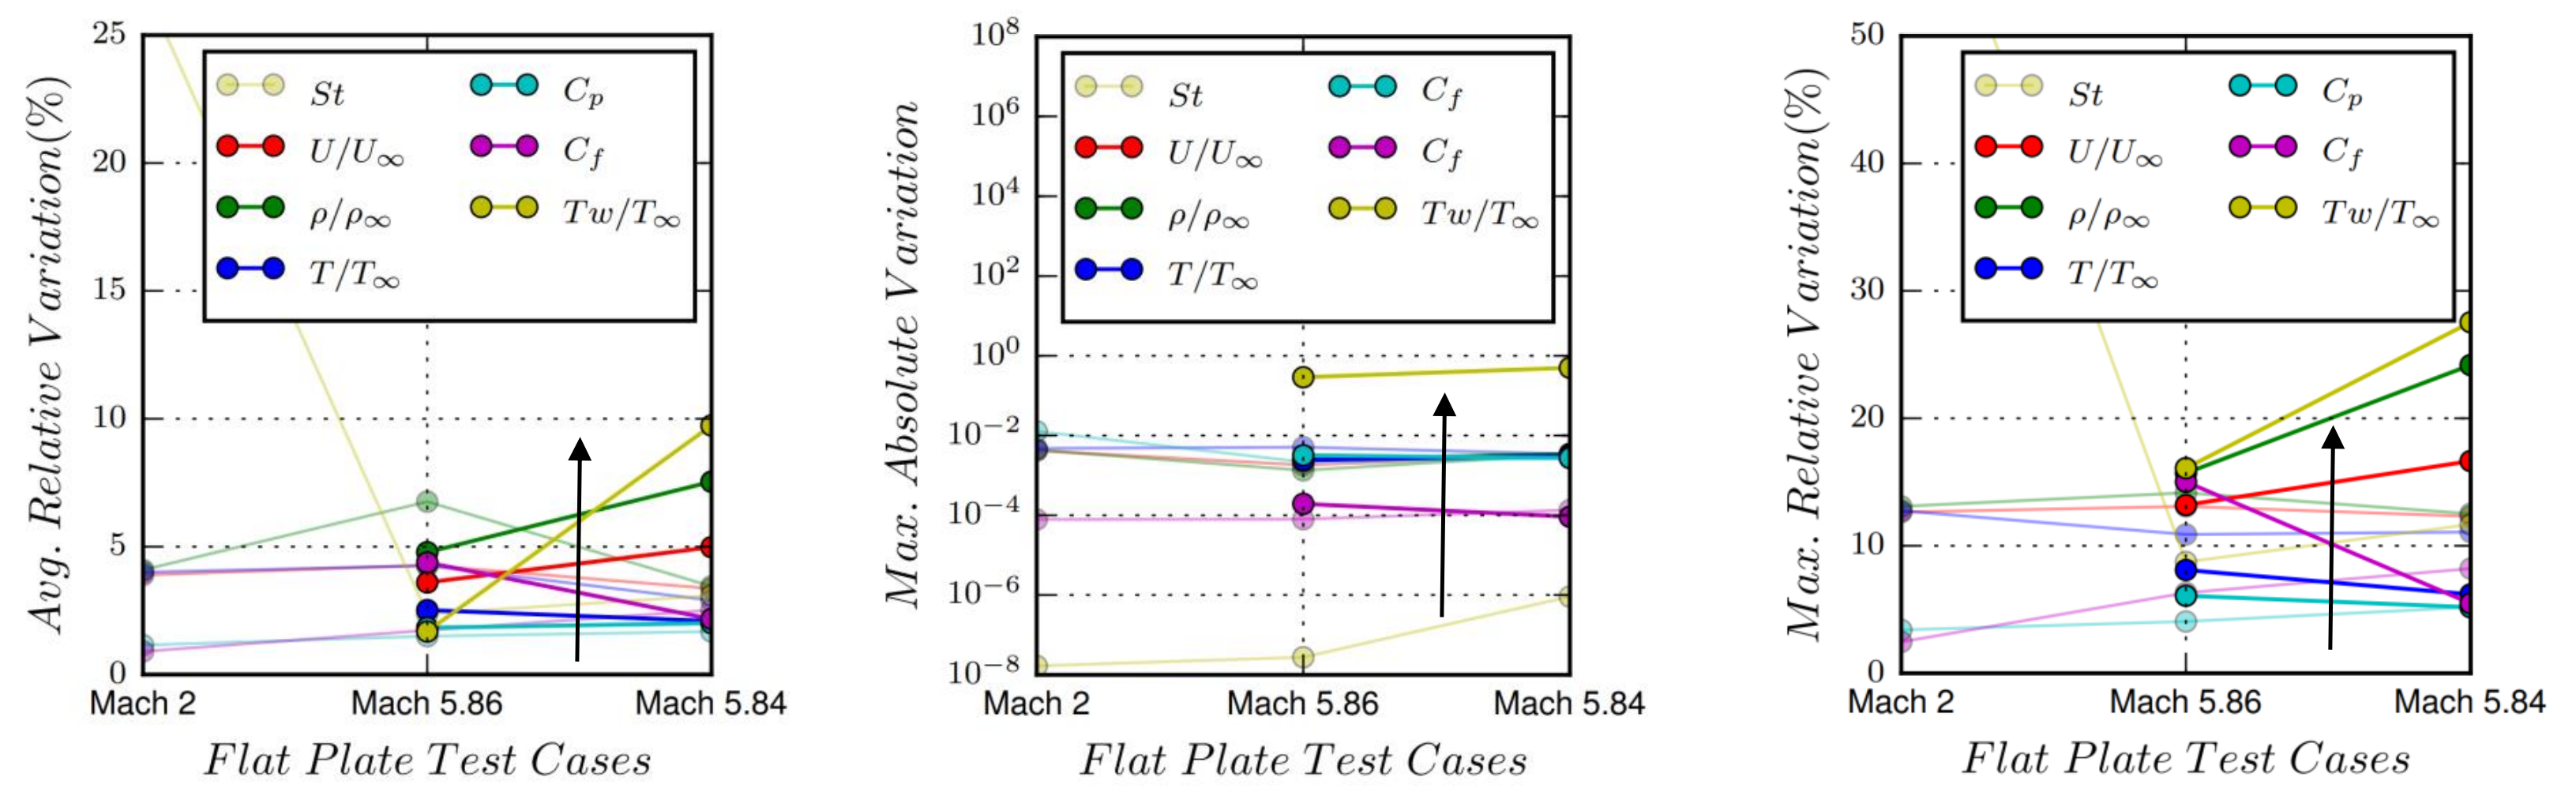
\includegraphics[width=\textwidth]{CHT/Avg_Rel_Variation.png}
  \caption{A graphical representation of the computed solver variation using Equations \eqref{eq:var_avg_rel}, \eqref{eq:var_max_abs} and \eqref{eq:var_max_rel}. Solver variation generally increases with a constant heat flux wall B.C. as compared to a constant temperature wall B.C.}
  \label{fig:numericalquantification}
\end{figure}

\subsection{Supersonic Wedge}
The impact on solver variation due to a slightly more complex geometry is assessed using the supersonic wedge case. The flow parameters are declared identical to the flat plate test cases, such that the only difference between the case setup is geometry. The results of \texttt{rhoCentralFoam} are omitted from the wedge plots and solver variation calculations because of instabilities and convergence issues -- partly caused due to the lack of available resources to optimally configure a case for highly non-adiabatic hypersonic flows. All the solvers are compared at $x=0.5$ from the leading edge. Figures \ref{fig:Wedge_RANS2}, \ref{fig:Wedge_RANS6AD}, and \ref{fig:Wedge_RANS6} show wall-normal solver comparison data for the supersonic wedge cases. The average integrated variation in the solvers is similar to the flat plate case, at around $2\%$ to $5\%$ (see Table \ref{tab:Wedge_ConstT_comp}). The supersonic wedge case results show that the maximum variation between the wall-normal profiles is generally reduced when compared to the flat plate cases. On the other hand, the wall quantities like coefficient of pressure, coefficient of skin friction, and wall-heat flux, in general, vary more than their flat plate counterparts. The same trend as in the flat plate case appears here in the wedge case results as well: in general, an increase in Mach number decreases solver variation, and an increasing wall cooling rates increases the variation between the solvers. Once again, these results are not conducive enough to claim a correlation between Mach number and wall cooling effects on solver variation, and a deeper investigation is needed in a later study. 


\section*{Acknowledgments}
This research was enabled in part by support provided by SharcNet, Scinet and Compute Canada (www.computecanada.ca). The research funding was provided by Mitacs through a collaboration with QinetiQ Target Systems. The work was initiated through discussions with Dr. Bryan Godbolt and Ed Farnfield.

\bibliography{sample,bibl_JPH}
\clearpage
\section*{APPENDIX}
\begin{figure}[h]
\centering
  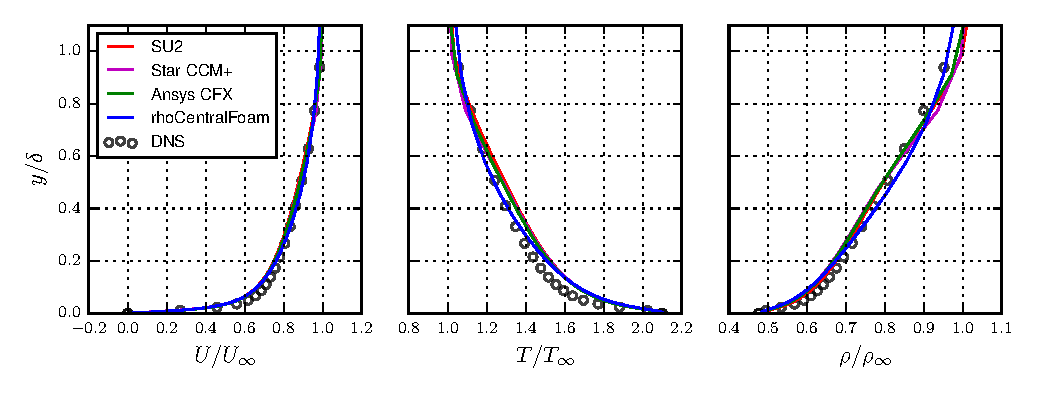
\includegraphics[width=0.9\textwidth]{figs/Plate_RANS2_Comp_new.pdf}
  \caption{Normalized wall-normal properties for Mach 2.5 supersonic wedge with high wall cooling ($T_w/T_{aw} = 1$), compared to DNS at $Re_\theta = 2825$.}
  \label{fig:Plate_RANS2}
\end{figure}

\begin{figure}[h]
\centering
  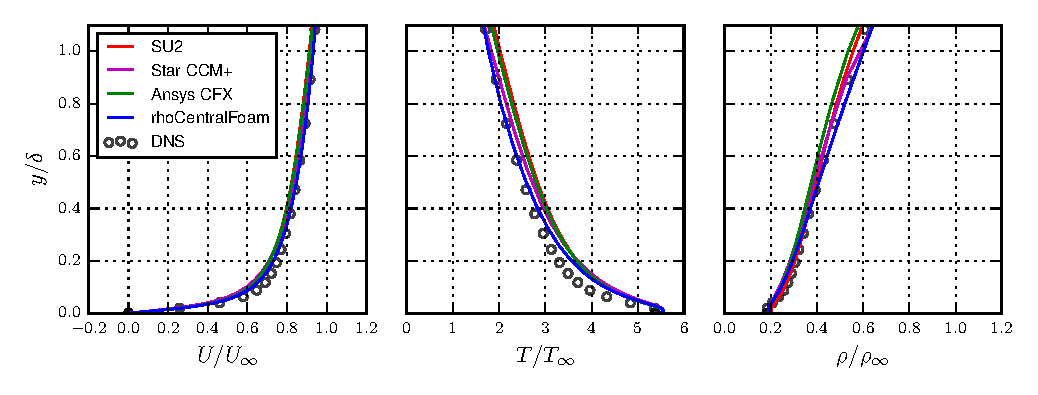
\includegraphics[width=0.9\textwidth]{figs/Plate_RANS6AD_Comp_new.pdf}
  \caption{Normalized wall-normal properties for Mach 5.86 supersonic wedge with low wall cooling ($T_w/T_{aw} = 0.76$), compared to DNS at $Re_\theta = 9455$.}
  \label{fig:Plate_RANS6AD}
\end{figure}

\begin{figure}[h]
\centering
  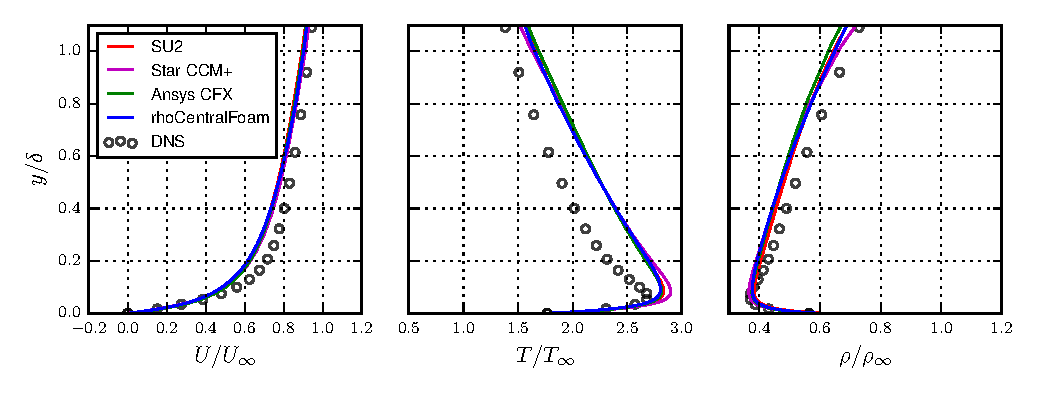
\includegraphics[width=0.9\textwidth]{figs/Plate_RANS6_Comp_new.pdf}
  \caption{Normalized wall-normal properties for Mach 5.84 supersonic wedge with high wall cooling ($T_w/T_{aw} = 0.25$), compared to DNS at $Re_\theta = 2121$.}
  \label{fig:Plate_RANS6}
\end{figure}

\begin{figure}
\centering
  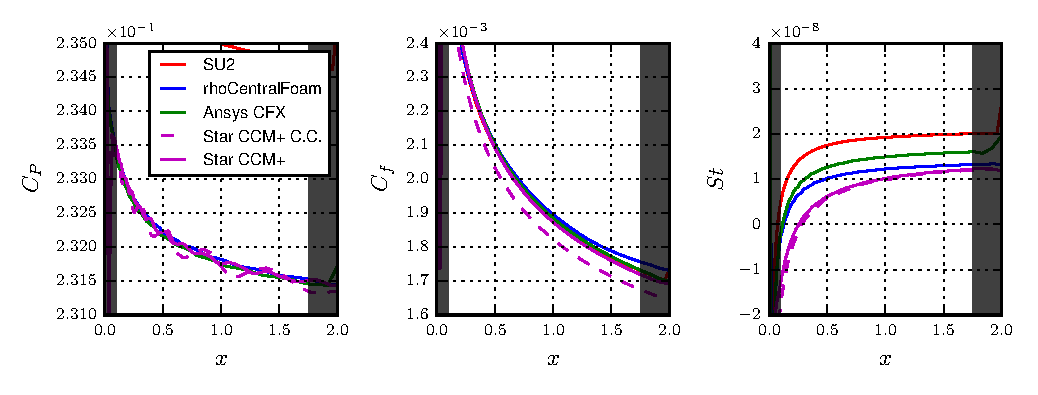
\includegraphics[width=0.9\textwidth]{figs/Plate_RANS2_Cd_new.pdf}
  \caption{Coefficient of pressure, coefficient of skin friction drag, and wall heat flux for Mach 2.5 supersonic flat plate with no wall cooling ($T_w/T_{aw} = 1$). The red marker shows the corresponding Stanton number for the DNS case at $Re_\theta = 2825$. The dotted line shows the effect of Sarkar's compressibility correction in Star-CCM+.}
  \label{fig:Plate_RANS2_Cd}
\end{figure}

\begin{figure}
\centering
  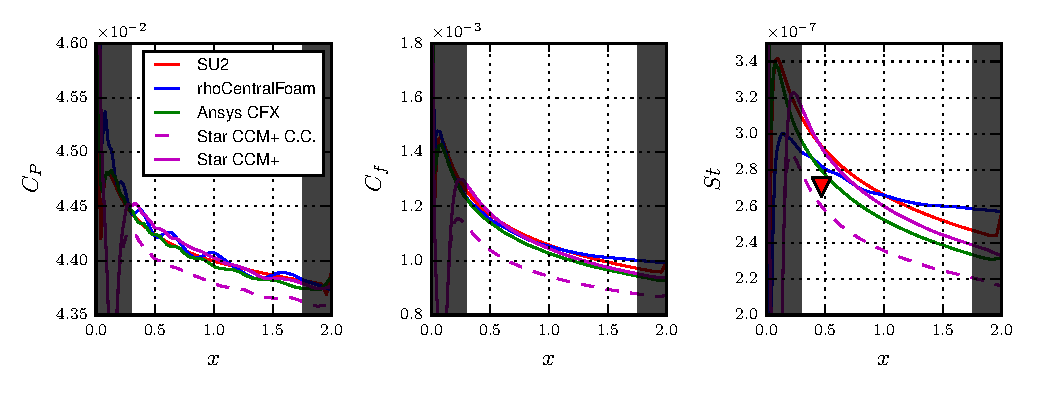
\includegraphics[width=\textwidth]{figs/Plate_RANS6AD_Cd_new.pdf}
  \caption{Coefficient of pressure, coefficient of skin friction drag, and wall heat flux for Mach 5.86 supersonic flat plate with low wall cooling ($T_w/T_{aw} = 0.76$). The red marker shows the corresponding Stanton number for the DNS case at $Re_\theta = 9455$. The dotted line shows the effect of Sarkar's compressibility correction in Star-CCM+.}
  \label{fig:Plate_RANS6AD_Cd}
\end{figure}

\begin{figure}
\centering
  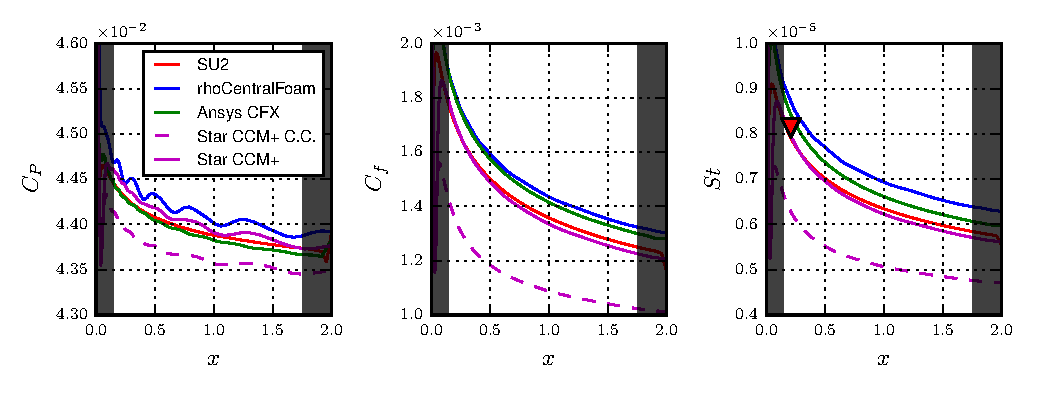
\includegraphics[width=\textwidth]{figs/Plate_RANS6_Cd_new.pdf}
  \caption{Coefficient of pressure, coefficient of skin friction drag, and wall heat flux for Mach 5.84 supersonic flat plate with high wall cooling ($T_w/T_{aw} = 0.25$). The dotted line shows the effect of Sarkar's compressibility correction in Star-CCM+.}
  \label{fig:Plate_RANS6_Cd}
\end{figure}
\end{document}

\begin{figure}[h]
\centering
  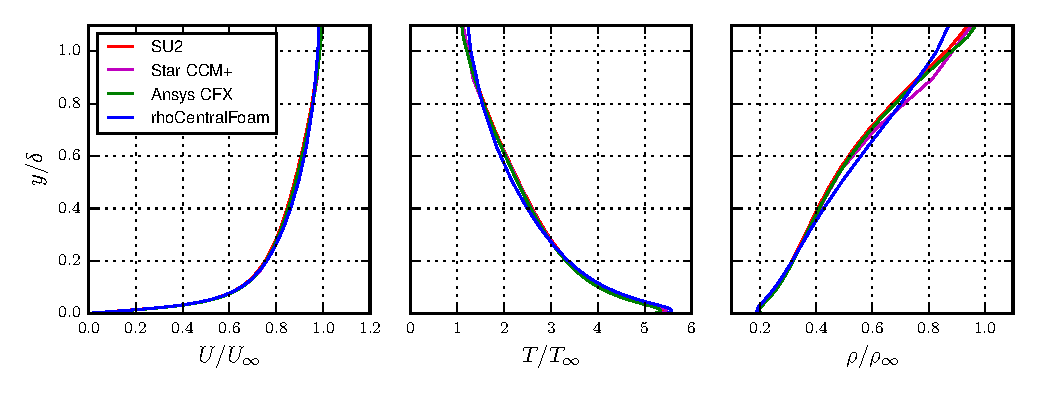
\includegraphics[width=\textwidth]{figures/Plate_RANS6HFLow_new.pdf}
  \caption{Normalized wall-normal properties for Mach 5.86 supersonic flat plate with low wall cooling with a constant heat flux boundary condition ($q_w = -2500 W/m^2$).}
  \label{fig:Plate_RANS6HFLow}
\end{figure}

\begin{figure}
\centering
  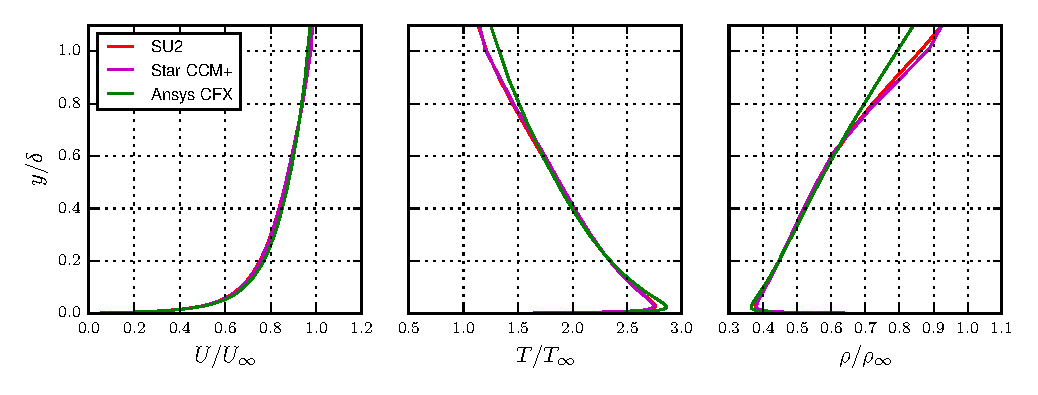
\includegraphics[width=\textwidth]{figures/Plate_RANS6HFHigh_new.pdf}
  \caption{Normalized wall-normal properties for Mach 5.84 supersonic flat plate with high wall cooling with a constant heat flux boundary condition ($q_w = -1000 W/m^2$).}
  \label{fig:Plate_RANS6HFHigh}
\end{figure}

\begin{figure}
\centering
  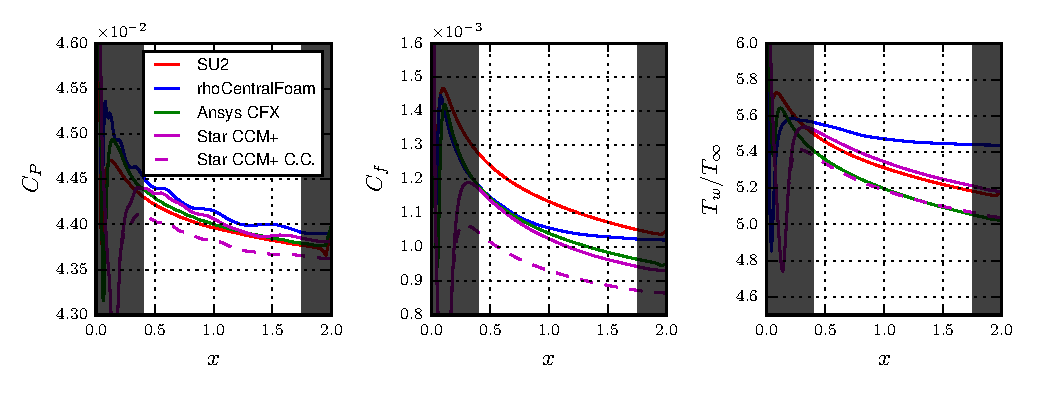
\includegraphics[width=\textwidth]{figures/Plate_RANS6HFLow_Cd_new.pdf}
  \caption{Coefficient of pressure, coefficient of skin friction drag, and normalized wall temperature for Mach 5.86 supersonic flat plate with low wall cooling ($q_w = -2,500 W/m^2$).}
  \label{fig:Plate_RANS6HFLow_Cd}
\end{figure}

\begin{figure}
\centering
  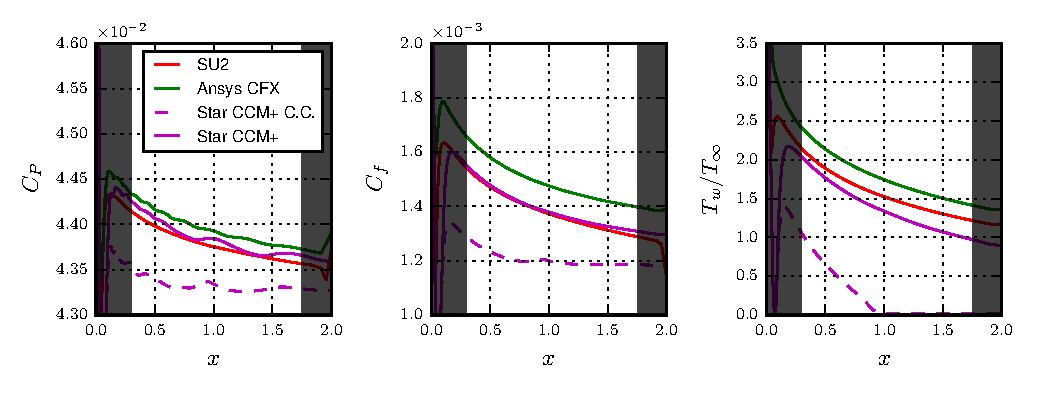
\includegraphics[width=\textwidth]{figures/Plate_RANS6HFHigh_Cd_new.pdf}
  \caption{Coefficient of pressure, coefficient of skin friction drag, and normalized wall temperature for Mach 5.84 supersonic flat plate with high wall cooling ($q_w = -10000 W/m^2$).}
  \label{fig:Plate_RANS6HFHigh_Cd}
\end{figure}